\chapter{Arquitecturas digitales para la implementación de sistemas MIMO}

En el capítulo anterior fueron expuestos los beneficios de la implementación de la técnica de \textit{beamforming} en los sistemas MIMO. Se llegó a la conclusión de que, para la implementación de un filtro de \textit{beamforming}, se requiere el cómputo una de matriz inversa. Para este objetivo, existen diferentes algoritmos. La elección del algoritmo adaptativo para derivar el vector de pesos es muy importante, dado que determina tanto la velocidad de convergencia como la complejidad de hardware requerido para implementar el algoritmo.

Existen dos algoritmos muy populares para resolver esta necesidad, \textbf{el algoritmo LMS} (\textit{Least Mean Squares}) y \textbf{el algoritmo RLS} (\textit{Recursive Least Squares}), entre otros, los cuales fueron abordados en el capítulo anterior. Entre los diferentes algoritmos, generalmente el algoritmo RLS es preferido por su propiedad de convergencia rápida.

Entre los diversos trabajos analizados, los cuales se mencionan en las últimas secciones de este capítulo, se encontró que en la gran mayoría de los casos el algoritmo implementado es el algoritmo RLS. Existen diversas formas de implementar las ecuaciones en hardware. Diferentes técnicas encontradas mencionan el uso del método de \textbf{Gram Schmidt}, las \textbf{transformaciones de Householder}, el método \textbf{Squared Givens Rotations} y las rotaciones de Givens. Las diferencias sustanciales entre los trabajos analizados se encuentran en la forma de implementar los procesadores de cómputo de las ecuaciones (CORDIC, squared givens rotations, Gram-Schmidt), el tipo de mapeo de la arquitectura junto con la cantidad de procesadores utilizados, y la forma de interconexión de los mismos.

En este capítulo, se abordarán los distintos tipos de arquitecturas existentes para la implementación de procesadores de descomposición QR.

\section{Resolución del algoritmo RLS}

El algoritmo RLS estándar requiere el cómputo explícito de una matriz de correlación \cite{Woods}. Este es un cálculo intensivo que tiene el efecto de elevar al cuadrado el número de condición del problema, causando un efecto negativo en la longitud de palabra para la estabilidad en sistemas de longitud de palabra finita. Los pesos pueden ser calculados en un modo más estable, evitando el cálculo de la matriz de correlación y su inversa al utilizar la \textbf{descomposición QR}, una forma de triangularización ortogonal con buenas propiedades numéricas.

\section{Descomposición QR}
\label{sec:descomposicion_qr}

Existe una familia de algoritmos RLS numéricamente estables y robustos que evolucionó en un rango de métodos de descomposición QR, tales como las rotaciones de Givens y las transformaciones de Householder. Las rotaciones de Givens son rotaciones ortogonales planas, utilizadas para eliminar elementos en una matriz. Al aplicar una serie de rotaciones de Givens sucesivas, una matriz puede ser triangularizada al eliminar los elementos debajo de la diagonal. Esta operación es conocida como factorización QR, en la cual una matriz $X(n)$ es descompuesta en una matriz triangular superior $R(n)$ y una matriz ortogonal $Q(n)$ (sus columnas son vectores unitarios ortogonales indicando que $Q^T Q = I$) de forma tal que:

\[
X(n) = Q(n)R(n)
\]

La matriz $X(n)$ de dimensión $P \times N$ es descompuesta en una matriz triangular superior $R(n)$ de dimensión $N \times N$ a través de la aplicación de una matriz unitaria $Q^T(n)$ de forma tal que:

\[
Q^T(n)X(n)=
	\left[ 
		\begin{array}{c}
			R(n) \\
			0
		\end{array}
	\right] 
\]

Donde 0 es la matriz cero que resulta si $N < P$. Debido a que $Q(n)$ es una matriz unitaria, entonces:

\[
\phi(n) = X^T(n)X(n) = X^T(n)Q(n)Q^T(n)X(n) = R^T(n)R(n)
\]

La matriz triangular, $R(n)$, es el factor Cholesky (raíz cuadrada) de la matriz de correlación de información $\phi(n)$. Debido a que $Q(n)$ es unitaria el sistema de ecuaciones original puede expresarse como:

\[
\| J(n) \| = \| Q(n)e(n) \| = \Big|\Big| \underbrace{Q^T(n)X(n)}_{R(n)}W_{LS}(n) + \underbrace{Q^T(n)y(n)}_{u(n)} \Big|\Big|
\]

Se sigue que el vector de cuadrados mínimos $ w_{LS}(n) $ debe satisfacer la ecuación:

\[
R(n)w_{LS}(n) + u(n) = 0
\]

Debido a que $ R(n)$ es una matriz triangular superior, los pesos pueden ser resueltos utilizando sustitución. Esta descomposición permite que la matriz sea triangularizada nuevamente cuando nueva información entra en la matriz, sin la necesidad de computar la triangularización desde el formato de matriz cuadrada original. La matriz de información $X(n)$ y el vector de medida $y(n)$ en un tiempo $n$ pueden ser representados en un modo recursivo a través de la matriz resultante previa y el vector de nueva información, de forma tal que:

\[
X(n)=
	\left[ 
		\begin{array}{c}
			\lambda(n)X(n-1) \\
			\underline{x}^T(n)
		\end{array}
	\right] 
\]

y

\[
y(n)=
	\left[ 
		\begin{array}{c}
			\lambda(n)y(n-1) \\
			\underline{y}(n)
		\end{array}
	\right] 
\]

donde $\underline{x}^T(n)$ e $\underline{y}^T(n)$ forman la fila concatenada en el tiempo $n$. Una forma de raíz cuadrada del algoritmo es lograda como sigue:

\[
Q^T(n)
	\left[ 
		\begin{array}{c}
			\lambda^{0.5} R(n-1)     \\
			\underline{x}^T(n) 
		\end{array}
	\right]
	W_{LS}(n) =
\]
\[
Q^T(n)
	\left[ 
		\begin{array}{c}
			\lambda^{0.5} u(n-1)     \\
			\underline{y}(n) 
		\end{array}
	\right]
	+ Q^T(n)e(n)
\]

donde $\beta = \lambda^{0.5}$. Luego, esto nos da:

\[
Q^T(n)
	\left[ 
		\begin{array}{cc}
			\beta(n)R(n-1)     & \beta(n)u(n-1)  \\
			\underline{x}^T(n) & \underline{y}(n)
		\end{array}
	\right] 
	=
	\left[ 
		\begin{array}{cc}
			R(n) & u(n)  \\
			0    & \alpha(n)
		\end{array}
	\right]
\]

Esto se computa para dar:

\[
	\left[ 
		\begin{array}{c}
			R(n) \\
			0    
		\end{array}
	\right] 
	W_{LS}(n)
	=
	\left[ 
		\begin{array}{c}
			u(n) \\
			\alpha(n)
		\end{array}
	\right]
\]

$\alpha(n)$ está relacionado con el residuo de cuadrados mínimos a posteriori, $e(n)$, en el tiempo $n$ de forma que:

\[
e(n) = \alpha(n)\gamma(n)
\]

donde $\gamma(n)$ es el producto de cosenos generado en el proceso de eliminar $\underline{x}^T(n)$.

El gráfico de dependencia a alto nivel en la realización de la solución QR para RLS se puede ver en la figura \ref{fig:dependence_graph}:

\begin{figure}[h!]
        \centering
        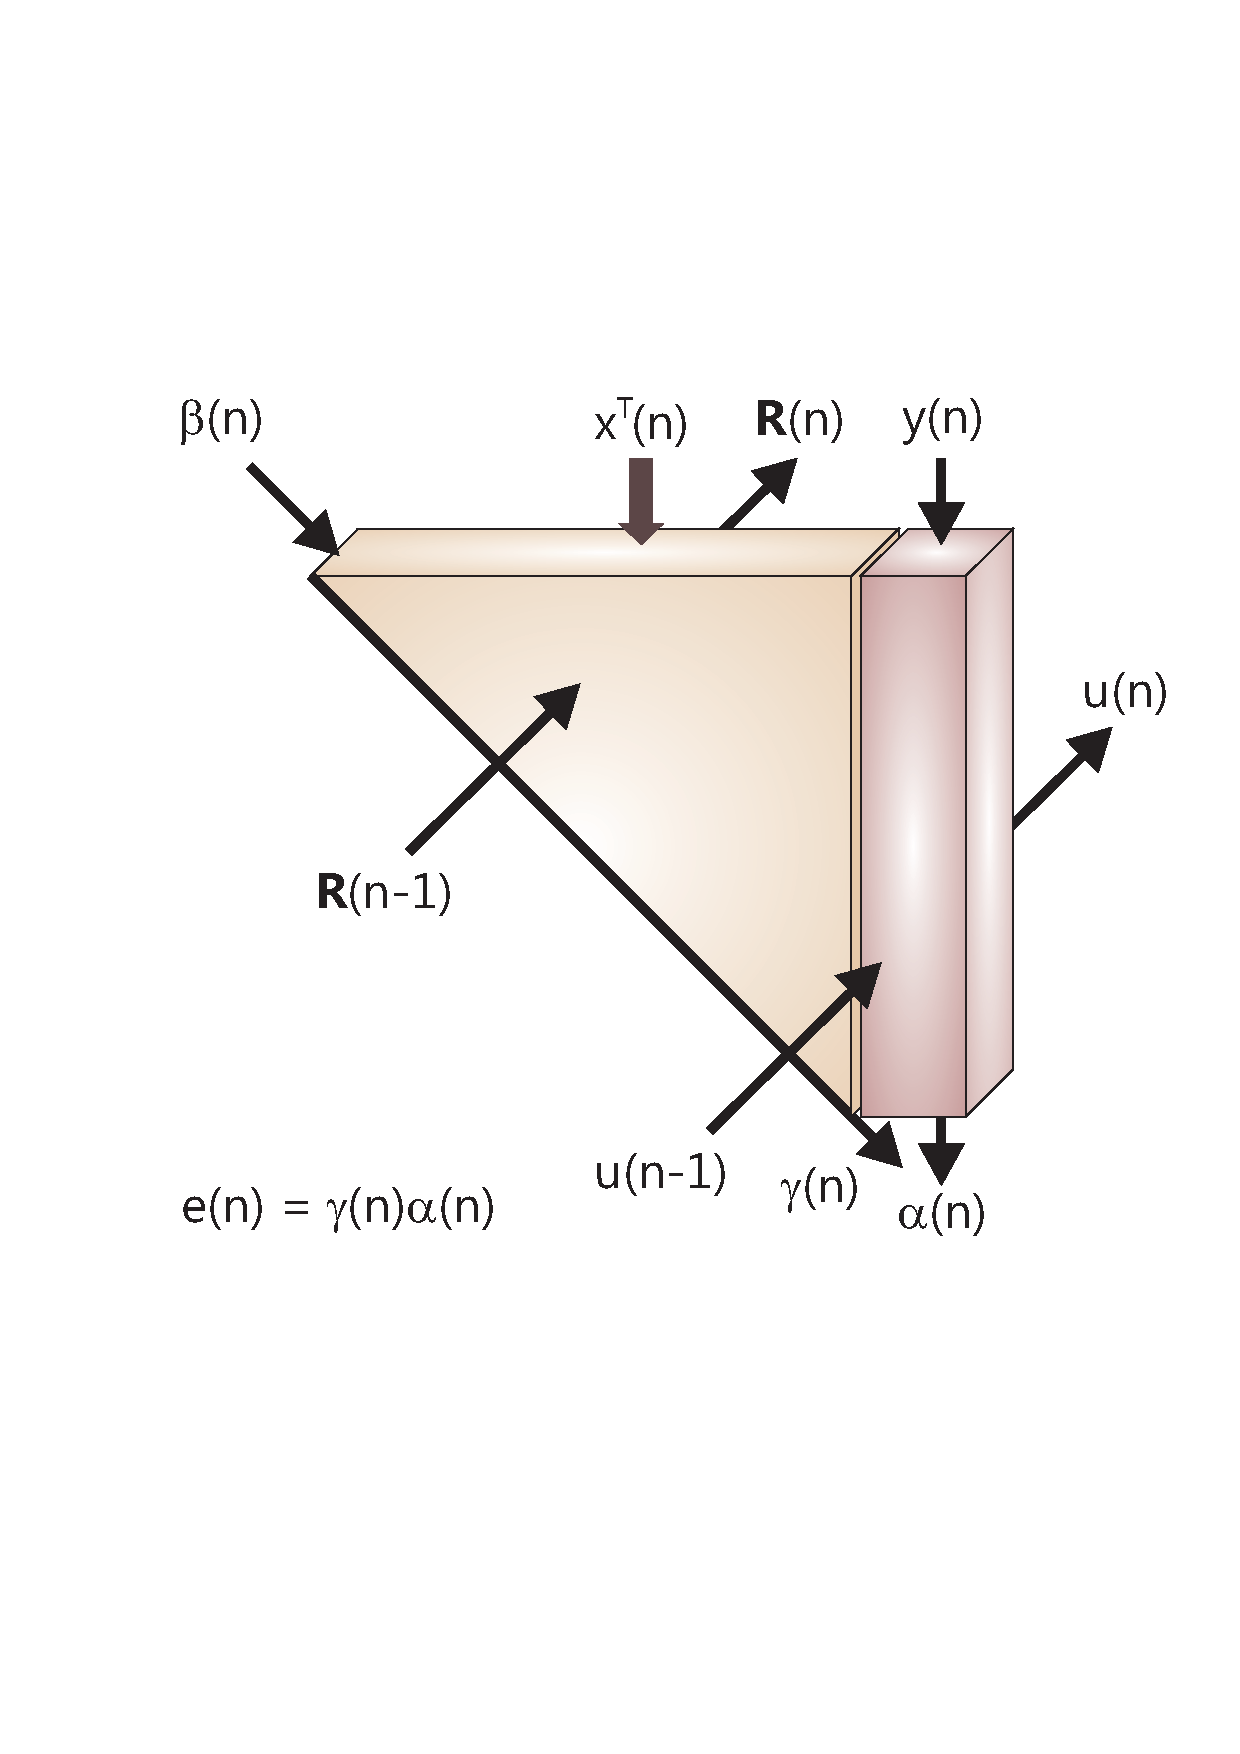
\includegraphics[width=6cm]{./figures/C03-dependence_graph}
        \caption{Gráfico de dependencias en alto nivel para la solución QR-RLS}
        \label{fig:dependence_graph}
\end{figure}

La matriz $X(n)$ es pre-multiplicada por matrices de rotación, un elemento a la vez. Los parámetros son calculados de forma que los elementos por debajo de la diagonal en la primera columna sean convertidos a cero. Luego se sigue con los elementos de la siguiente columna, hasta que la matriz triangular superior equivalente es conformada.

Givens logra esta operación a través de una secuencia de rotaciones, que se pueden explicar utilizando el siguiente ejemplo para una matriz de $2\times3$:

\[
M=
	\left[
		\begin{array}{ccc}
			a_{11} & a_{12} & a_{13} \\
			a_{21} & a_{22} & a_{23}
		\end{array}
	\right]
\]

La matriz es transformada en una matriz pseudo-triangular al eliminar el elemento $a_{21}$. Esto se logra a través de la multiplicación de la siguiente matriz de rotación con la matriz $M$:

\[
G=
	\left[
		\begin{array}{cc}
			 \cos\alpha & -\sin\alpha\\
			 \sin\alpha &  \cos\alpha
		\end{array}
	\right]
\]

Luego:

\[
	\left[
		\begin{array}{cc}
			 \cos\alpha & -\sin\alpha\\
			 \sin\alpha & \cos\alpha
		\end{array}
	\right]
	\left[
		\begin{array}{ccc}
			a_{11} & a_{12} & a_{13} \\
			a_{21} & a_{22} & a_{23}
		\end{array}
	\right]
	= 
\]
\[
	\left[
		\begin{array}{ccc}
			 a_{11}\cos\alpha-a_{21}\sin\alpha &
			 a_{12}\cos\alpha-a_{22}\sin\alpha &
			 a_{13}\cos\alpha-a_{23}\sin\alpha \\
			 a_{11}\sin\alpha+a_{21}\cos\alpha &
			 a_{12}\sin\alpha+a_{22}\cos\alpha &
			 a_{13}\sin\alpha+a_{23}\cos\alpha
		\end{array}
	\right]
\]

Para eliminar $a_{21}$ se debe resolver $a_{11}\sin\alpha+a_{21}\cos\alpha = 0$. Luego, por trigonometría, se puede plantear la siguiente solución:

\begin{align}
\cos\alpha &=  a_{11} / \sqrt{a_{11}^2 + a_{21}^2}\\
\sin\alpha &= -a_{21} / \sqrt{a_{11}^2 + a_{21}^2}\\
 a_{11new} &= \sqrt{a_{11}^2 + a_{21}^2}\\
 a_{21new} &= 0
\end{align}

Aplicando la rotación para eliminar $a_{21}$ resulta en la matriz pseudo-triangular:

\[
M=
	\left[
		\begin{array}{ccc}
			a_{11new} & a_{12new} & a_{13new} \\
			    0     & a_{22new} & a_{23new}
		\end{array}
	\right]
\]

Esta función puede implementarse en un arreglo sistólico, como se ve en la figura \ref{fig:rls_givens_rotations}, el cual consiste en dos tipos de celdas, referidas como \textit{boundary cell} (BC - representada con un círculo) e \textit{internal cell} (IC - representada con un cuadrado).

\begin{figure}[h!]
        \centering
        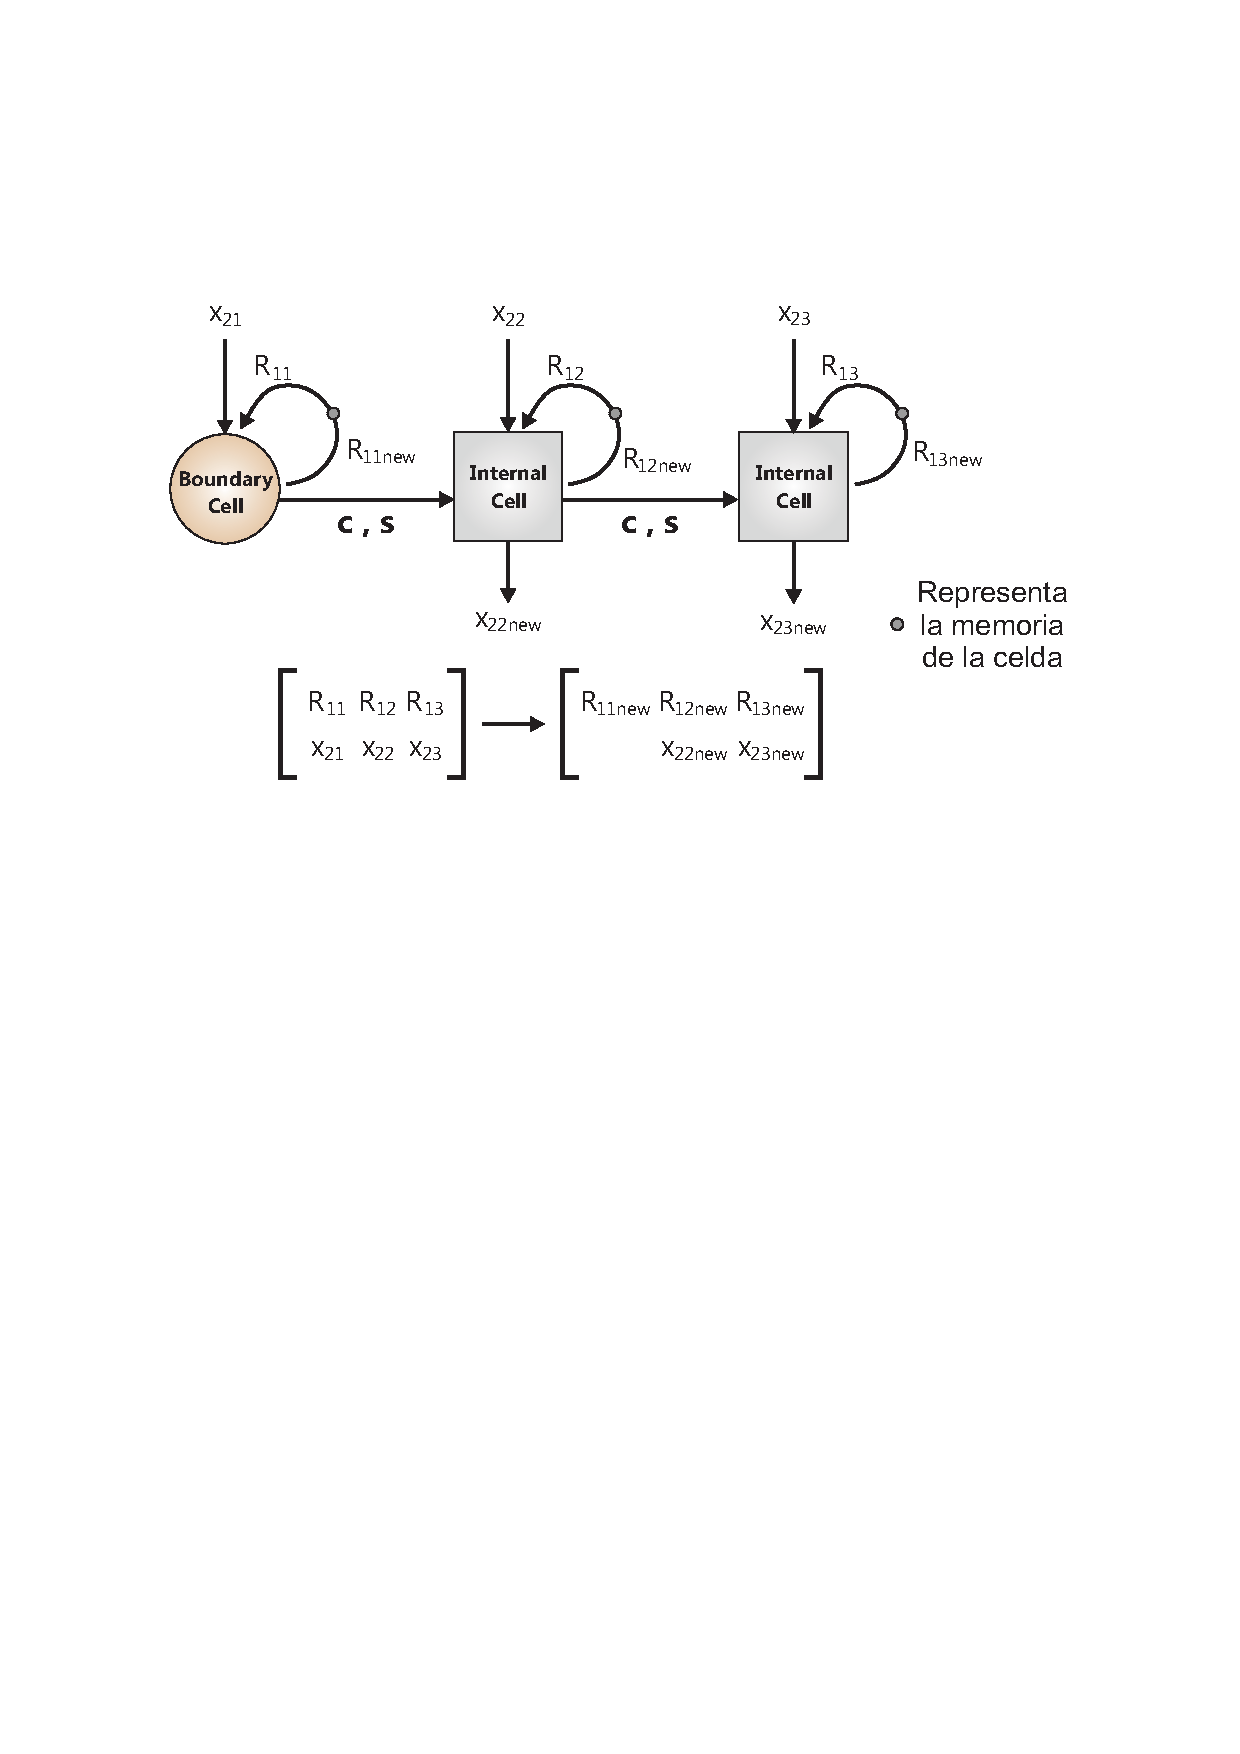
\includegraphics[width=10cm]{./figures/C03-rls_givens_rotations}
        \caption{Transformación por Rotaciones de Givens}
        \label{fig:rls_givens_rotations}
\end{figure}

Los elementos en los cuales se aplican las rotaciones son $x$ y $R$, donde $x$ es el valor de entrada en la celda, y $R$ es el valor retenido en la memoria para esa celda. Los parámetros de rotación, $\cos\alpha$ y $\sin\alpha$, son calculados en una \textit{boundary cell}, de forma tal que el valor de $x$ que ingresa a una \textit{boundary cell} sea convertido a 0, y el valor de R de dicha celda sea actualizado acorde a la rotación y almacenado para la próxima iteración.

Los parámetros de rotación son enviados sin modificar a lo largo de toda una fila a cada una de las \textit{internal cells} para continuar con la rotación. El gráfico de dependencia de la figura \ref{fig:rls_givens_rotations} representa la eliminación de $x_{21}$, relacionado con el elemento de la matriz $a_{21}$ del ejemplo anterior. Los valores de $R$ y $x$ son considerados una coordenada polar $(R, x)$.

Eliminar la entrada $x$ en una \textit{boundary cell}, se logra a través de rotar el vector un ángulo $\alpha$ tal que:

\[
R_{new} = R \cos\alpha - x \sin\alpha = \frac{R^2 + x^2}{\sqrt{R^2 + x^2}} = \sqrt{R^2 + x^2}
\]

donde

\[
\cos\alpha = \frac{R}{R_{new}} = c
\hspace{3cm}
\sin\alpha = \frac{-x}{R_{new}} = s
\]

Los mismos parámetros de rotación utilizados en BC son aplicados en las ICs:

\[
R_{new} = cR - sX \hspace{3 cm}
x_{new} = cx + sR
\]

Al concatenar rotaciones de Givens sucesivas, la factorización QR puede ser implementada para una matriz $N \times N$. El diagrama de la figura \ref{fig:givens_for_3x3} muestra un ejemplo para una matriz de $3 \times 3$. Se trata de un esquema \textit{pipeline} en el cual los valores de R son realimentados a sus propias celdas para la próxima iteración.

\begin{figure}[h!]
        \centering
        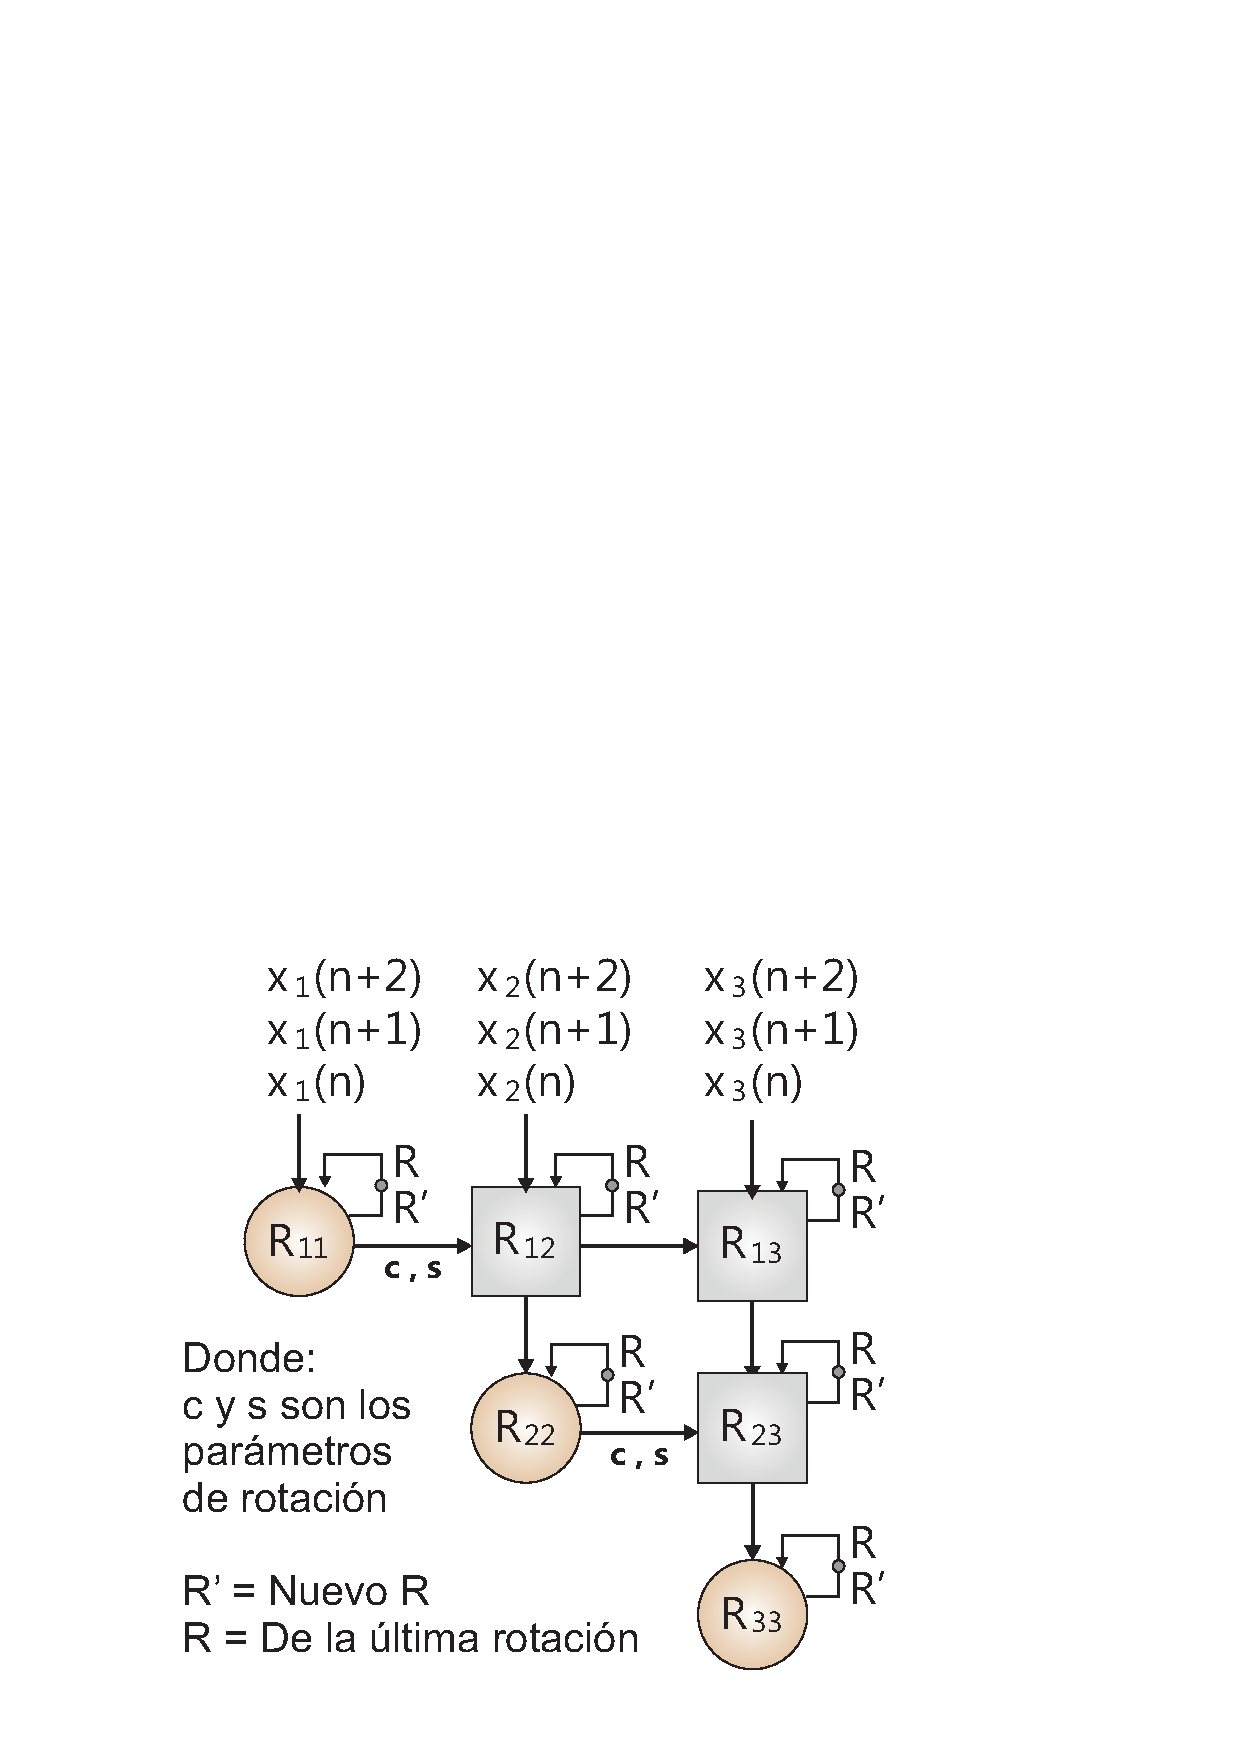
\includegraphics[width=5cm]{./figures/C03-givens_for_3x3}
        \caption{Descomposición QR aplicada a una matriz de 3x3}
        \label{fig:givens_for_3x3}
\end{figure}

A continuación se explorará en un nivel más detallado el proceso de desarrollar una arquitectura en hardware desde el algoritmo RLS y sus ecuaciones resuelto por descomposición QR utilizando rotaciones de Givens.

\section{Del algoritmo a una arquitectura sintetizable}

Con el objetivo de lograr la implementación, es necesario transformar las ecuaciones presentadas en una arquitectura sintetizable. En este proceso, es un aspecto clave el lograr una implementación de un circuito de alta \textit{performance}, para asegurar una traducción eficiente del algoritmo a hardware en silicio. Esto normalmente conlleva el hecho de desarrollar una arquitectura en la cual operaciones independientes se desarrollen en paralelo para aumentar el rendimiento.

En la figura \ref{fig:development_process} se presenta el proceso de transformar las ecuaciones a un procesador en hardware.

\begin{figure}[h!]
        \centering
        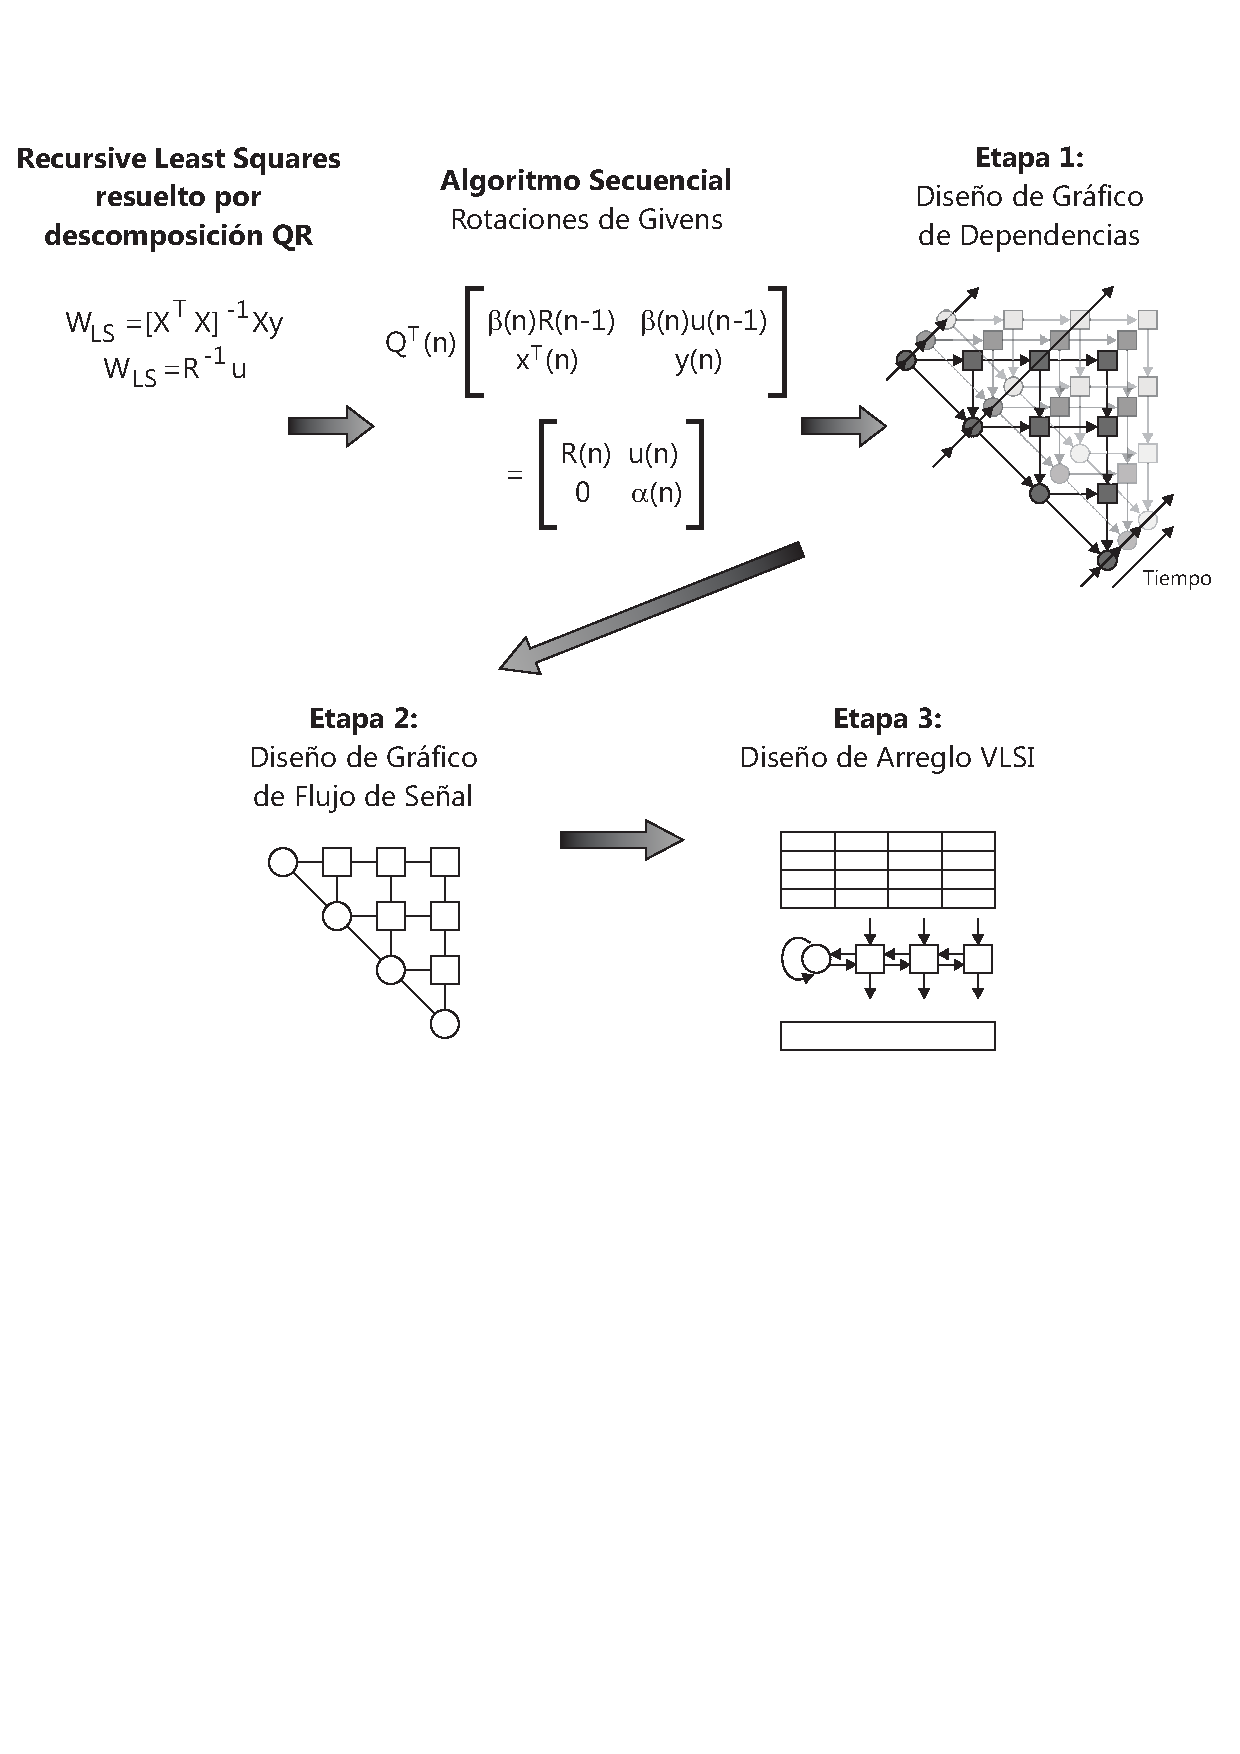
\includegraphics[width=14cm]{./figures/C03-development_process}
        \caption{Proceso de desarrollo del circuito digital}
        \label{fig:development_process}
\end{figure}

El punto de inicio en la figura es la resolución del algoritmo RLS a través de la descomposición QR. La siguiente etapa muestra dicha resolución a través del uso de un algoritmo secuencial. Esto es, por cada iteración del algoritmo, un nuevo conjunto de valores ingresa a las ecuaciones y evoluciona a una nueva solución.

La operación QR puede representarse como un arreglo triangular de operaciones. La matriz de información es la entrada en la parte superior del triángulo, y en cada fila son eliminados los términos para resultar en una matriz triangular superior.

El gráfico de dependencias en la figura \ref{fig:development_process} expone este proceso de triangularización. Los arreglos triangulares en cascada representan \textbf{cada iteración en el tiempo}. Las flechas muestran la dependencia a través del tiempo. Desde el diagrama de dependencias, se desarrolla posteriormente un diagrama de flujo de señal adecuado, y con el mismo se deriva una arquitectura sintetizable.

\subsection{Gráfico de dependencias}

En este diagrama se pueden detectar las dependencias entre los datos, permitiendo identificar el máximo nivel de concurrencia posible al desensamblar el algoritmo en nodos y flechas. Los nodos representan los cálculos y la dirección de las flechas la dependencia de las operaciones. En la figura \ref{fig:dependence_vs_signal} se muestra un ejemplo de $3 \times 3$. Cada esquema en perspectiva representa una iteración en el tiempo (para $n$, $n+1$ y $n+2$). Las flechas demuestran que, por ejemplo, para hacer el cálculo de $a_{12}$, se requiere la salida del procesamiento realizado en $a_{11}$, o que para hacer el cálculo de $a_{22}$, se requiere la salida de los procesamientos realizados en $a_{11}$ y $a_{12}$.

\begin{figure}[h!]
        \centering
        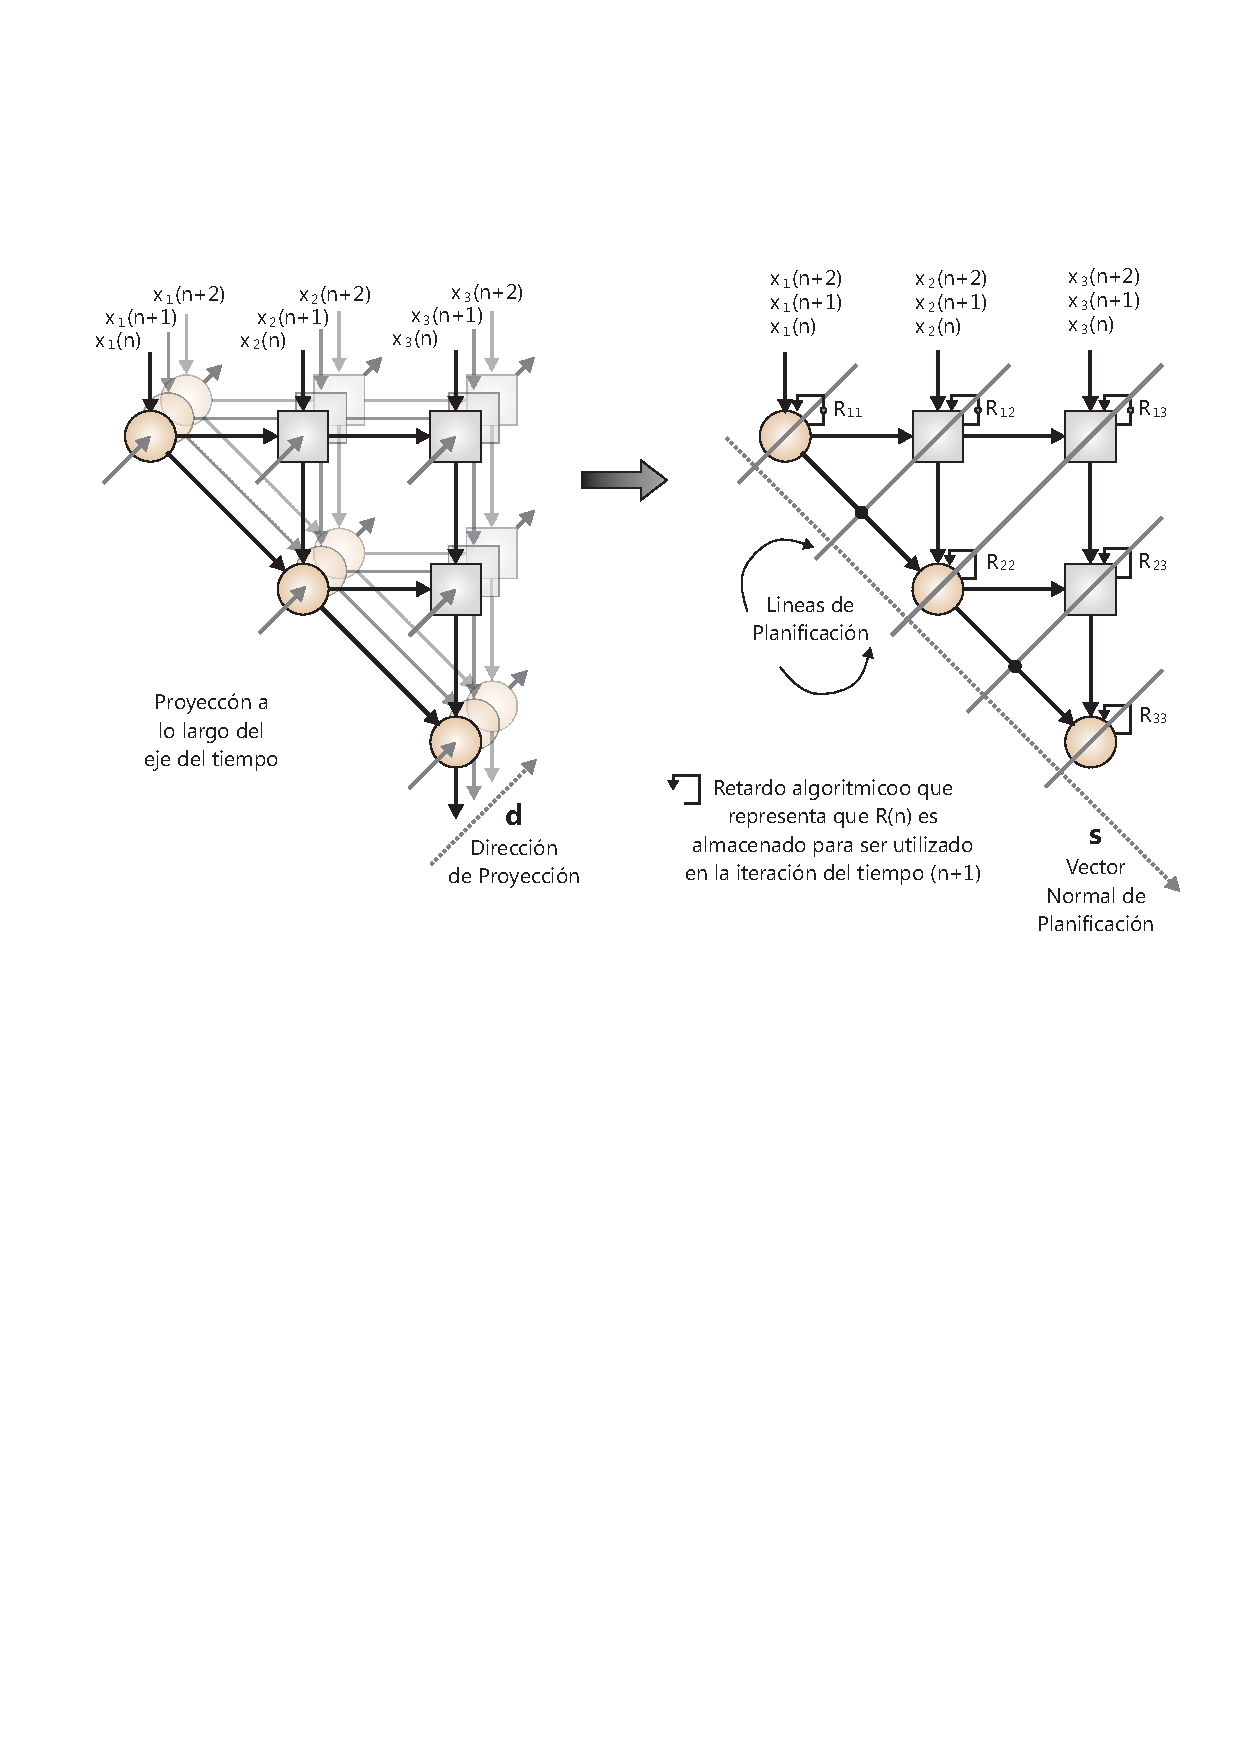
\includegraphics[width=12cm]{./figures/C03-dependence_vs_signal}
        \caption{Gráfico de Dependencias y Gráfico de Flujo de Señal}
        \label{fig:dependence_vs_signal}
\end{figure}

\subsection{Gráfico de flujo de señal}

En la figura \ref{fig:dependence_vs_signal}, se puede observar la transición del gráfico de dependencias al gráfico de flujo de señal. Este es el gráfico de mayor importancia para derivar a una arquitectura, dado que representa el sentido en el cual deben transmitirse las señales, y el orden en el cual se deben realizar las operaciones. Los nodos del gráfico de dependencias son asignados a procesadores, y sus operaciones son planificadas entre los mismos.

Una de las formas más sencillas para lograr esta transición es \textbf{la proyección lineal de todos los nodos idénticos} a lo largo de una linea recta en un único procesador. Esto es representado por el vector de proyección $\mathbf{d}$. La planificación lineal es utilizada para determinar el orden en el cual las operaciones son realizadas en estos procesadores. Las \textbf{líneas de planificación} en la figura \ref{fig:dependence_vs_signal} \textbf{indican las operaciones que se pueden realizar en paralelo} en cada ciclo de reloj. Matemáticamente están representadas por un \textbf{vector de planificación} $\mathbf{s}$ normal a las líneas de planificación, el cual apunta en la dirección de la dependencia de las operaciones (muestra el orden en el cual cada línea de operaciones es realizada).

Existen dos reglas que gobiernan la proyección y la planificación:

\begin{itemize}
	\item[•] Todos los arcos de dependencia fluyen en la misma dirección a lo largo de las líneas de planificación.
	\item[•] Las líneas de planificación no son paralelas con el vector de proyección $\mathbf{d}$.
\end{itemize}

En el ejemplo QR, cada arreglo triangular de celdas en el diagrama de dependencias representa una actualización QR. Al estar en cascada, el diagrama representa una \textbf{secuencia de actualizaciones QR}. Al proyectar a lo largo del eje del tiempo, todas las actualizaciones QR pueden ser asignadas a un diagrama de flujo de señal triangular, como se observa en la imagen.

Los valores $R$ son transmitidos a lo largo del tiempo de una actualización QR a la otra, representados por la cascada de arreglos triangulares. Esta transición se observa mejor en el diagrama de flujo de señal en la realimentación de los valores $R$ en la celda a partir de un \textit{delay} algorítmico utilizado para retener los valores hasta la próxima iteración. Esto es referido como un lazo recursivo.

La simplicidad del diagrama de flujo de señal es que asume que todas las operaciones en los nodos ocupan un único ciclo, así como los \textit{delays} algorítmicos, representados por pequeños círculos oscuros. Estos \textit{delays} algorítmicos particionan las iteraciones del algoritmo y son una parte necesaria del mismo. El resultado del diagrama de flujo de señal es una representación más concisa del algoritmo con respecto al diagrama de dependencias.

El camino a seguir, una vez definido el diagrama de flujo de señal, es derivar una arquitectura eficiente e implementar en hardware el algoritmo.

\newpage

\section{Implementación sistólica de las rotaciones de givens}

A partir del gráfico de flujo de señal, se debe profundizar el mismo a un nivel de detalle que defina la forma en la cual se implementarán los procesadores, la cantidad de los mismos que van a ser utilizados, la forma en la cual se almacenarán los datos, y cómo se realizará el control de los mismos. Existen diferentes mapeos desarrollados para derivar del arreglo triangular una arquitectura sintetizable. Veremos a continuación algunos de ellos.

\subsection{Mapeo de Gentleman y Kung}
\label{sec:mapeo_de_gentleman_y_kung}

El modo más directo de transformar el algoritmo en una arquitectura sintetizable consiste en la implementación de un arreglo sistólico en el cual cada \textit{boundary cell} e \textit{internal cell} sea calculada por un procesador independiente. Dicho esquema se presenta en la figura \ref{fig:direct_mapping}. 

\begin{figure}[h!]
        \centering
		\begin{minipage}[b]{0.4\textwidth}
			\footnotesize
			\[ [x_1(n) x_2(n) x_3(n)] = \underline{x}^T(n) \]
			\[ \left[
					\begin{array}{ccc}
						R_{11}(n-1) & R_{12}(n-1) & R_{13}(n-1) \\
							        & R_{22}(n-1) & R_{23}(n-1) \\
							        & 			  & R_{33}(n-1)
					\end{array}
				\right] = R(n-1) \]
			\[ \left[
					\begin{array}{c}
						u_{14}(n-1) \\
						u_{24}(n-1) \\
						u_{34}(n-1)
					\end{array}
				\right] = u(n-1) \]\vspace{1 cm}\\
			\normalsize
		\end{minipage}%
		\begin{minipage}[b]{0.6\textwidth}
        	\centering
        	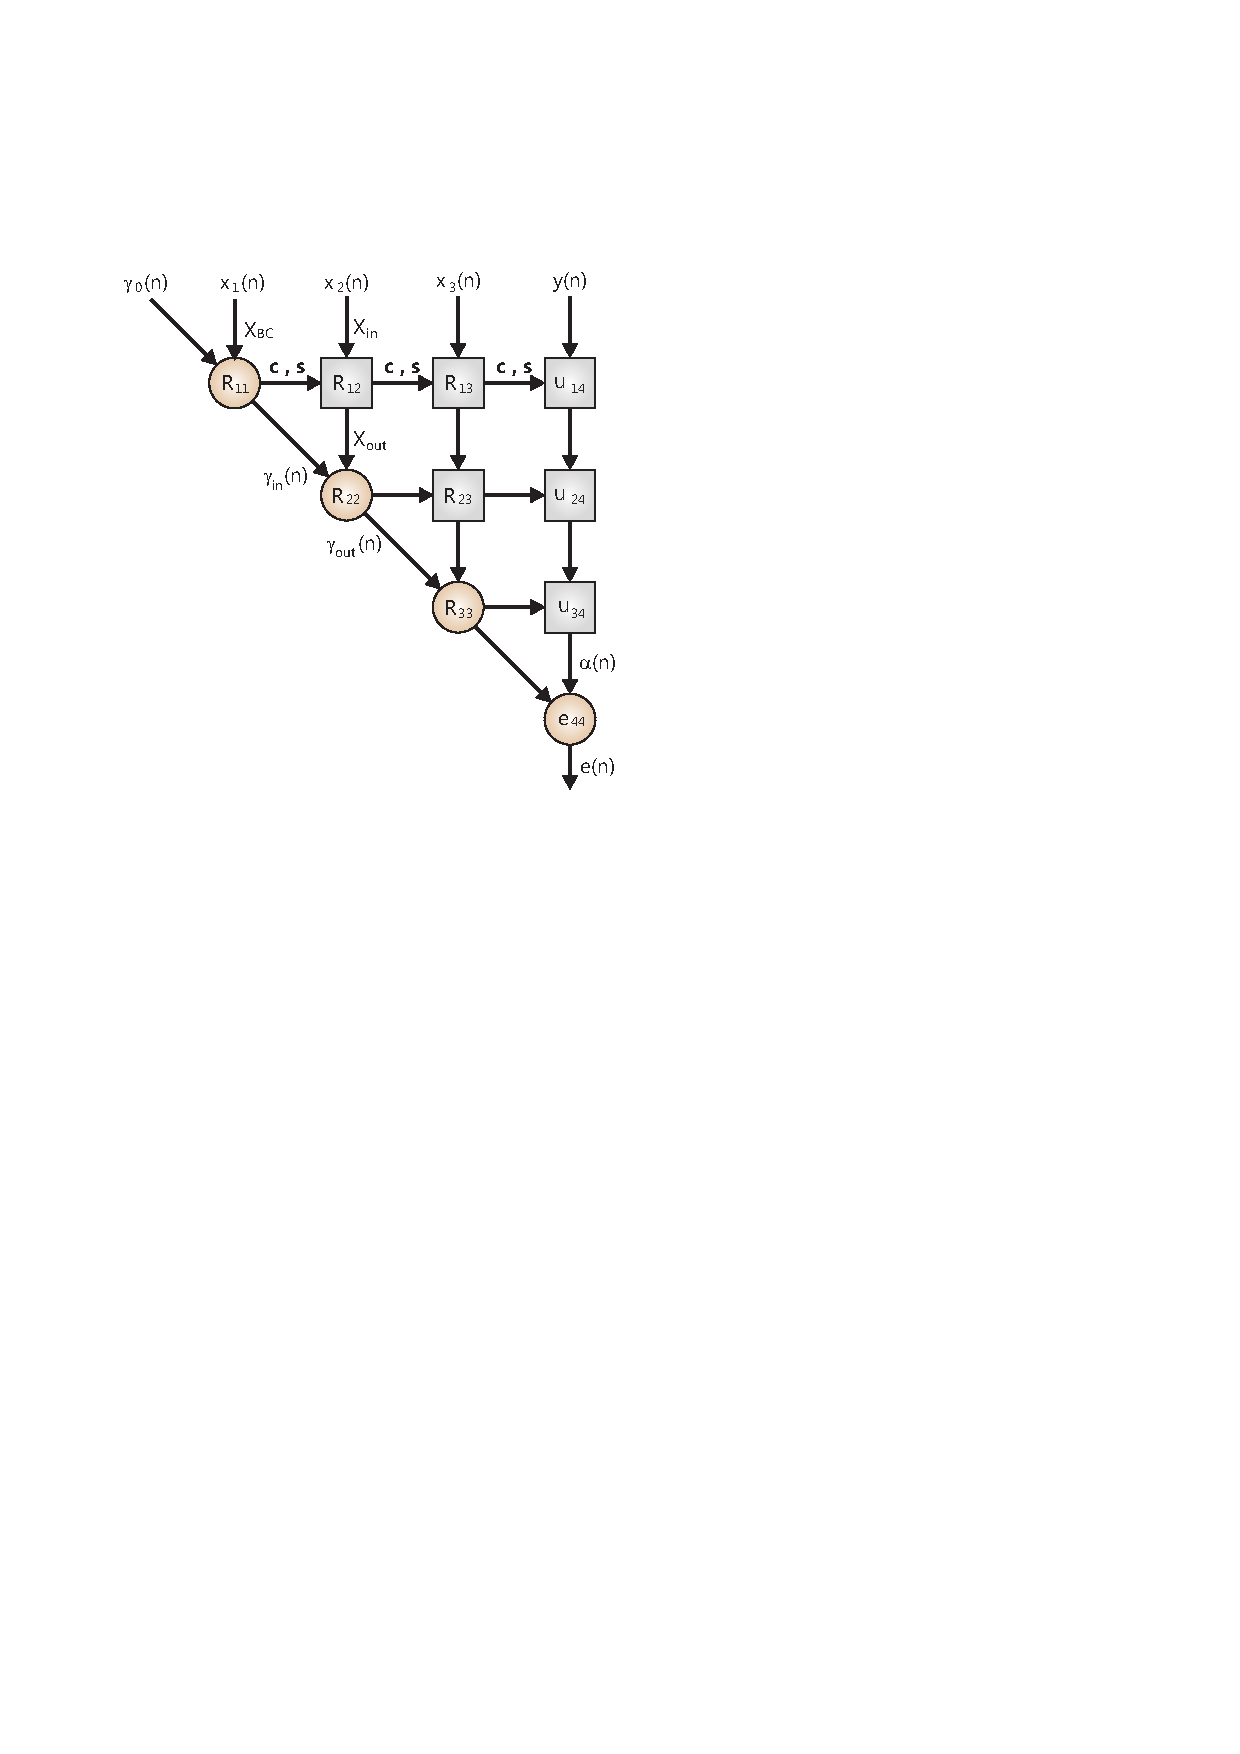
\includegraphics[width=6cm]{./figures/C03-direct_mapping}
        \end{minipage}%
        \caption{Esquema de mapeo directo}
        \label{fig:direct_mapping}
\end{figure}

Esta arquitectura fue desarrollada por Gentleman y Kung y modificada por McWhirter. En la misma, el vector de información $\mathbf{x}^T(n)$ ingresa al sistema desde la parte superior del arreglo y es progresivamente eliminado al computar la rotación en cada fila de la matriz en proceso. Los parámetros $c$ y $s$ son calculados en una BC de forma que eliminen la entrada $x_{i,i}(n)$. Estos parámetros son posteriormente enviados a las ICs de la misma fila para actualizar las componentes según el resultado de la rotación aplicada. Los valores de salida de las ICs $x_{i+1,j}(n)$ se convierten en los valores de entrada para la próxima fila. Al mismo tiempo, una nueva entrada ingresa en la parte superior del arreglo y el proceso se repite. En el proceso, los valores de $R(n)$ y $u(n)$ son actualizados para registrar la rotación y luego almacenados en el arreglo para ser utilizados en el próximo ciclo.

Para el algoritmo RLS, la implementación del factor de olvido $\lambda$ y el producto de cosenos $\gamma$ debe ser incluido en las ecuaciones. Por lo tanto, las operaciones de BC e IC son modificadas acordemente. Una notación es asignada a las variables en el arreglo. Cada término $R$ y $u$ posee un sub-índice denotado por (i,j), que representa la ubicación de los elementos en la matriz $R$ y el vector $u$. Una notación similar es asignada a las entradas $X$ y a las variables de salida. Las descripciones de las celdas para las BCs e ICs son presentadas en las figuras \ref{fig:direct_mapping_2} y \ref{fig:direct_mapping_3} respectivamente.

\begin{figure}[h!]
        \centering
        \begin{minipage}[b]{0.4\textwidth}
        	\centering
            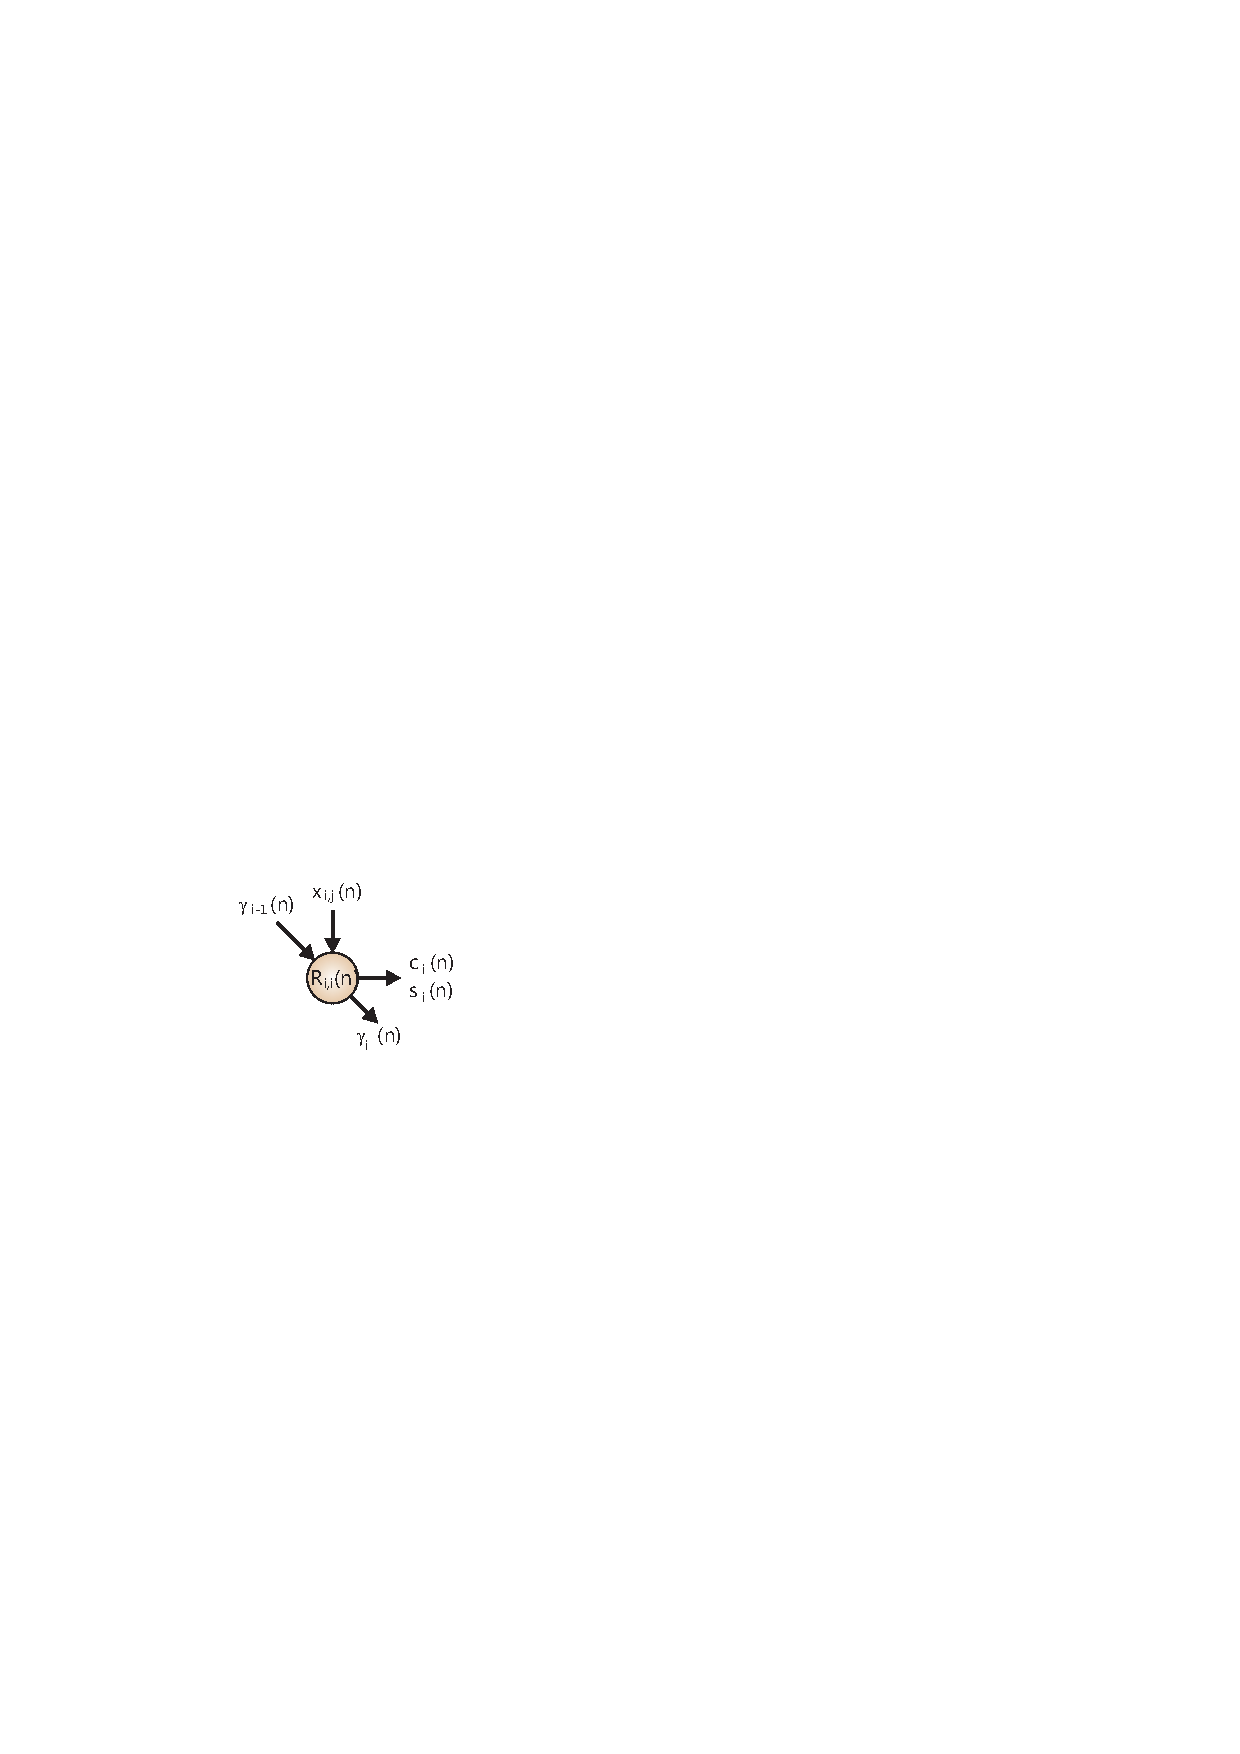
\includegraphics[width=3 cm]{./figures/C03-bc}
            \caption{Boundary Cell}
            \label{fig:direct_mapping_2}
        \end{minipage}%
		\begin{minipage}[b]{0.6\textwidth}
			\small
			\begin{equation}
			\label{eq:boundary_cell_1}
			R_{i,i}(n) = \sqrt{\beta^2 R_{i,i}^2(n-1) + x^2_{i,i}(n)}
			\end{equation}
			\begin{equation}
			\label{eq:boundary_cell_2}
			c_i(n) = \beta \frac{R_{i,i}(n-1)}{R_{i,i}(n)}
			\end{equation}
			\begin{equation}
			\label{eq:boundary_cell_3}
			s_i(n) = \frac{x_{i,i}(n-1)}{R_{i,i}(n)}
			\end{equation}
			\[ \gamma_i(n) = c_i(n) \gamma_{i-1}(n-1) \]
			\normalsize
		\end{minipage}%
\end{figure}

\begin{figure}[h!]
        \centering
        \begin{minipage}[b]{0.4\textwidth}
        	\centering
            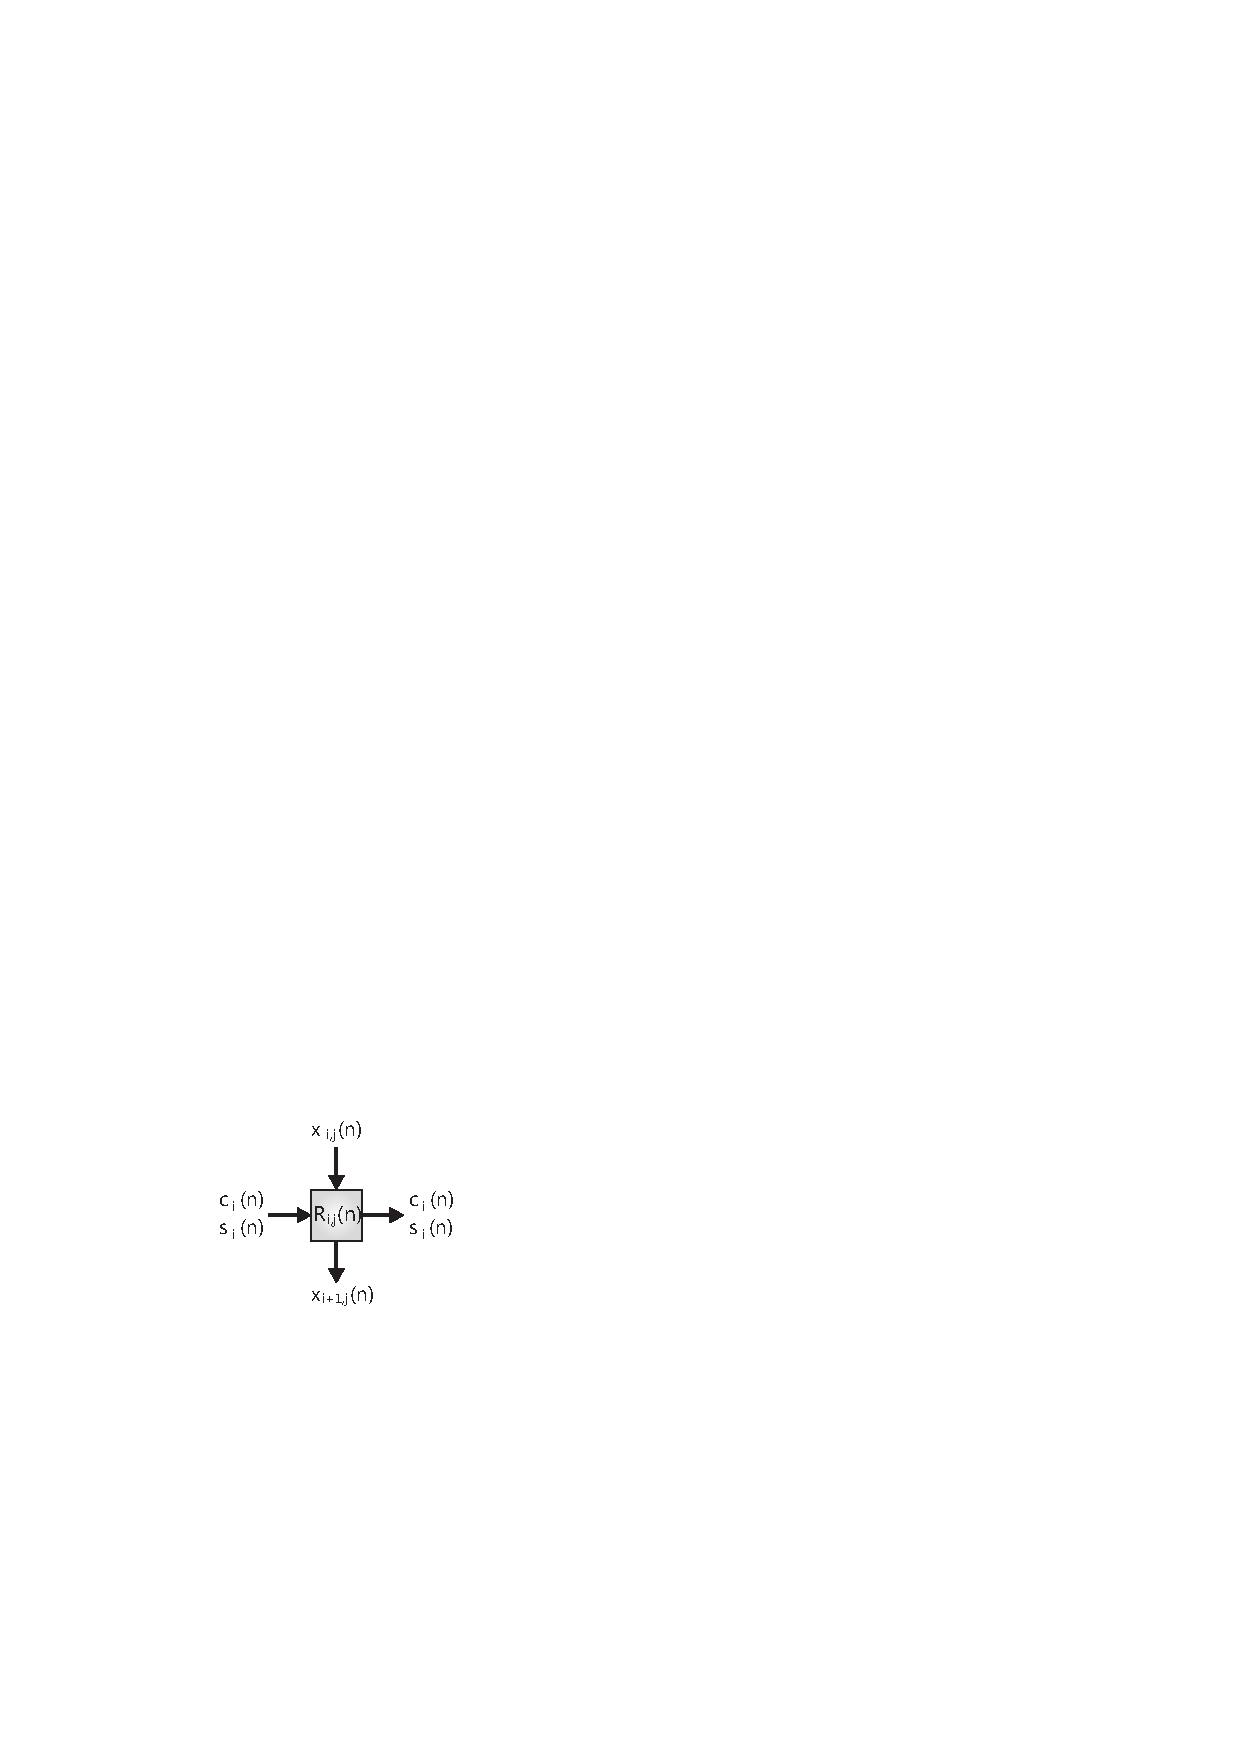
\includegraphics[width=3 cm]{./figures/C03-ic}
            \caption{Internal Cell}
            \label{fig:direct_mapping_3}
        \end{minipage}%
		\begin{minipage}[b]{0.6\textwidth}
			\small
			\begin{equation}
			\label{eq:internal_cell_1}
			x_{i+1,j}(n) = c_i(n) x_{i,j}(n) - s_i(n) \beta R_{i,j}(n-1)
			\end{equation}
			\begin{equation}
			\label{eq:internal_cell_2}
			R_{i,j}(n) = c_i(n) \beta R_{i,j}(n-1) + s_i(n) x_{i,j}(n)
			\end{equation} \\
			\normalsize
		\end{minipage}%
\end{figure}

Se puede destacar que, si bien la implementación de este mapeo es simple y es posible lograr que las celdas operen en un esquema \textit{pipeline}, la implementación requiere una gran cantidad de procesadores (en el ejemplo se tienen 10 para una matriz de $4 \times 4$) por lo cual ocupará un alto porcentaje de recursos del FPGA comparada con otras.

\subsection{Mapeo de proyección horizontal}

En la figura \ref{fig:horizontal_mapping} se puede observar un ejemplo de un mapeo de celdas QR en una arquitectura lineal proyectando de izquierda a derecha en N procesadores. Existen dos conflictos con dicho mapeo.

\begin{figure}[h!]
        \centering
        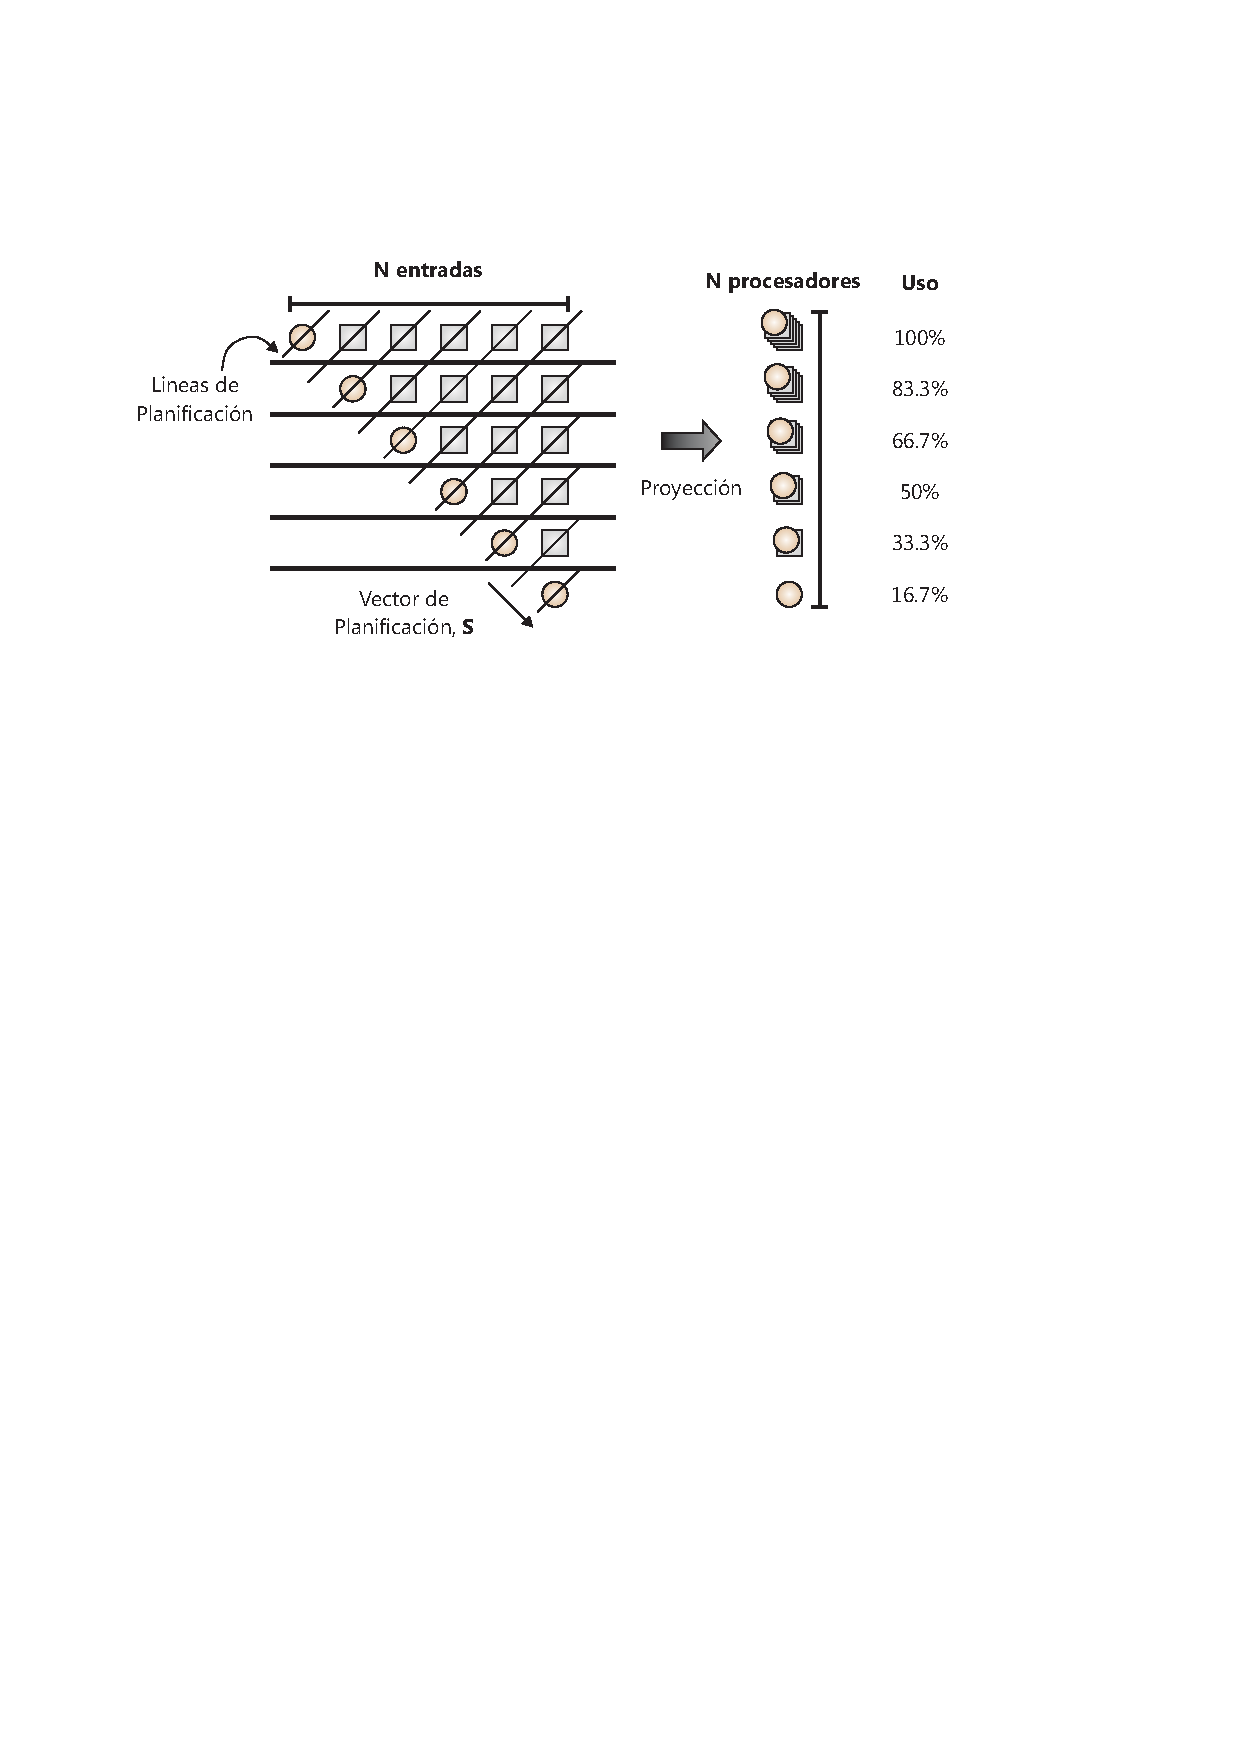
\includegraphics[width=13cm]{./figures/C03-horizontal_mapping}
        \caption{Esquema de Mapeo de Proyección Horizontal}
        \label{fig:horizontal_mapping}
\end{figure}

En primer lugar, tanto las operaciones de BC como de IC están mapeadas en un mismo procesador. De la figuras \ref{fig:direct_mapping_2} y \ref{fig:direct_mapping_3} se puede observar que existen diferencias entre dichas operaciones. En segundo lugar, los procesadores de la arquitectura mapeada no son utilizados eficientemente, siendo únicamente el primero aprovechado a máxima capacidad. La eficiencia se reduce en la columna de procesadores, llevando a una eficiencia total en la región del $60\%$, lo cual no es un óptimo uso de recursos.

\newpage

\subsection{Mapeo de Rader}

Rader (1992,1996) produjo una arquitectura eficiente al manipular la forma triangular, antes de asignar las operaciones a procesadores, como se observa en la figura \ref{fig:rader_mapping}.

\begin{figure}[h!]
        \centering
        \includegraphics[width=13cm]{./figures/C03-rader_mapping}
        \caption{Esquema de Mapeo de Rader}
        \label{fig:rader_mapping}
\end{figure}

La parte B del arreglo QR es espejada en el eje x y luego este resultado es espejado en el eje y para resultar en un arreglo de celdas rectangular que puede ser mapeado hacia abajo en una arquitectura lineal que consta de N/2 procesadores. Se puede observar que este mapeo presenta una mejora con respecto al mapeo de proyección horizontal, dado que los $N/2$ procesadores son utilizados el $100\%$ del tiempo. De todas maneras, los procesadores aun deben realizar ambas operaciones QR (BC e IC). Una opción para implementar este mapeo, es el uso de CORDIC, que logra arquitecturas similares tanto para BC como para IC.

\subsection{Mapeo de Walke}
\label{subsec:mapeo_de_walke}

Otro mapeo (Walke 1997 \cite{Walke}), logra una arquitectura eficiente al mantener las operaciones BC e IC en procesadores diferentes. Esto es logrado al manipular el arreglo triangular de forma inteligente a través de diversas transformaciones para alinear todas las operaciones BC en una columna y el resto de las operaciones IC en otras.

Dichas transformaciones constan de doblar, espejar y rotar las partes del arreglo QR. Las mismas se explicarán en el siguiente ejemplo para un arreglo triangular de 7 entradas. El resultado mapea un arreglo triangular de $2m^2+3m+1$ celdas ($N=2m+1$ entradas) en una arquitectura lineal, con interconexiones locales, consistiendo de un único procesador BC y $m$ procesadores IC, todos utilizados al 100\% de eficiencia.

Los pasos a seguir para obtener el arreglo rectangular son los siguientes:

\begin{enumerate}
	
	\item El arreglo triangular inicial es dividido en en dos triángulos más chicos A y B. El corte A es realizado luego de la BC $m+1^{ava}$ en una línea perpendicular a la diagonal de BCs.

	\begin{figure}[h!]
        \centering
        \includegraphics[width=14cm]{./figures/C03-walke_mapping_1}
        \caption{Esquema de Mapeo de Walke - Primera Transformación}
        \label{fig:walke_mapping_1}
	\end{figure}
	
	\item El triángulo B debe ser manipulado para que pueda formar la parte superior del arreglo rectangular. Esto se logra en dos pasos. Al espejar el triángulo B en el eje x primero, las BCs son alineadas de forma que sean paralelas a las BCs en el triángulo A, formando un paralelogramo, como se observa en la figura \ref{fig:walke_mapping_2}. El triángulo espejado B es luego movido hacia arriba a lo largo del eje y, hacia la izquierda en el sentido del eje x, para posicionarse en la parte superior de A, formando el arreglo rectangular. Como se puede observar, las operaciones BC están alineadas en dos columnas, por lo cual el arreglo rectangular debe ser aún modificado para ser adecuado para una proyección lineal.

	\begin{figure}[h!]
        \centering
        \includegraphics[width=14cm]{./figures/C03-walke_mapping_2}
        \caption{Esquema de Mapeo de Walke - Segunda Transformación}
        \label{fig:walke_mapping_2}
	\end{figure}

	\item La siguiente etapa apunta a plegar el arreglo rectangular, de forma que las dos columnas de operaciones BC sean posteriormente alineadas a lo largo de una única. Este pliegue logra que las dos columnas de operaciones BC sean alineadas a izquierda.

	\begin{figure}[h!]
        \centering
        \includegraphics[width=14cm]{./figures/C03-walke_mapping_3}
        \caption{Esquema de Mapeo de Walke - Tercera Transformación}
        \label{fig:walke_mapping_3}
	\end{figure}

	\item  El último paso, consiste en intercalar las celdas de forma tal que se produzca un arreglo rectangular compacto. De este arreglo rectangular de procesador, se puede producir una arquitectura reducida al proyectar hacia abajo de la diagonal a un arreglo lineal, con todas las operaciones BC asignadas a un procesador de BC, y todas las operaciones de IC asignadas a una fila de $m$ procesadores IC (ver figura \ref{fig:walke_mapping_4}).

	\begin{figure}[h!]
        \centering
        \includegraphics[width=14cm]{./figures/C03-walke_mapping_4}
        \caption{Esquema de Mapeo de Walke - Cuarta Transformación}
        \label{fig:walke_mapping_4}
	\end{figure}
\end{enumerate}

La arquitectura lineal resultante se muestra con mayor detalle en la figura \ref{fig:walke_mapping_5}. Cada fila de procesadores dentro del arreglo rectangular de operaciones en la figura sigue la planificación vista anteriormente bajo la definición del vector de planificación o de \textit{schedule} $\mathbf{s}$, una flecha perpendicular a las líneas de planificación.

En esta etapa del análisis, se considera que cada celda de procesamiento toma un ciclo de \textit{clock}. Existen registros presentes en todas las salidas de las celdas de procesamiento del arreglo lineal resultante para mantener la planificación. Se colocan multiplexores en las entradas de las celdas QR para controlar la entrada de datos, sea de las entradas del sistema o de las celdas adyacentes.

Los multiplexores inferiores definen las diferentes direcciones del flujo de datos que ocurre entre filas y el arreglo original. Las celdas QR del arreglo original guardan los valores de R de una iteración a la siguiente. Este mismo almacenamiento también necesita ser realizado en la arquitectura reducida, requiriendo entonces almacenar un número de valores $R$ entre ciclos recursivos de celda por múltiples ciclos de \textit{clock}.

Una solución es \textbf{mantener los valores localmente} dentro de los caminos de datos recursivos de las celdas QR, en lugar de utilizar una memoria externa. Los valores son almacenados en registros locales para retrasarlos hasta que sean necesarios.

\newpage

\begin{figure}[h!]
     \centering
     \includegraphics[width=12cm]{./figures/C03-walke_mapping_5}
     \caption{Mapeo de Walke - Iteraciones}
     \label{fig:walke_mapping_5}
\end{figure}

\subsection{Planificación de las operaciones QR}

La derivación de la arquitectura es sólo una parte del desarrollo necesario. Una tarea más compleja es la determinación de una planificación válida que asegure que la información requerida para cada set de operaciones esté disponible en el momento de ejecución, mientras se siga manteniendo la eficiencia.

El arreglo rectangular de procesamiento de la figura \ref{fig:walke_mapping_5} contiene todas las operaciones requeridas por el algoritmo QR, mostrando la secuencia en la cual se van a implementar en la arquitectura lineal. Por lo tanto, este diagrama puede ser utilizado para mostrar la planificación de las operaciones a ser realizadas en el diagrama lineal. Al ver la primera línea de planificación, se puede observar que las operaciones de \textbf{dos actualizaciones diferentes} han sido intercaladas. Las celdas oscurecidas representan la actualización QR actual en tiempo $n$, y las no oscurecidas representan la actualización QR anterior no terminada, en tiempo $n-1$. Efectivamente, las actualizaciones QR han sido intercaladas. La primera operación QR empieza en el ciclo $= 1$, luego después de $2m + 1$ ciclos de la arquitectura lineal, la siguiente operación QR empieza. De la misma forma, luego de $2m + 1$ ciclos, la tercera operación QR es iniciada. En total, toma $4m + 1$ ciclos de la arquitectura lineal para completar la primera actualización QR, y $2m + 1$ las siguientes.

Las celdas QR necesitan tener la posibilidad de tomar las entradas de $x$ desde entradas externas del sistema, por ejemplo, desde muestras de información, formando la entrada de la matriz $x(n)$ y el vector $y(n)$, como se observa en la figura \ref{fig:walke_mapping_5}. Las entradas externas son alimentadas en la arquitectura lineal cada $2m + 1$ ciclos de reloj. Las mismas también van a tomar entradas que son internas al arreglo lineal.

Si cada celda QR toma un único ciclo de \textit{clock} para producir una salida, luego no existirá una violación a la planificación expuesta en la figura \ref{fig:dependence_vs_signal}. De todas formas, se deben realizar análisis adicionales dado que las celdas QR poseen requerimientos de \textit{timing} detallados. Un análisis de \textit{timing} de mayor profundidad es realizado en el Capítulo 5.

\section{Implementación de las operaciones BC e IC}

\subsection{El algoritmo CORDIC}
\label{subsec:El_algoritmo_CORDIC}

El algoritmo CORDIC provee un método iterativo para realizar rotaciones de vectores en diferentes ángulos utilizando únicamente sumas y desplazamientos \cite{Andraka}. El algoritmo, acreditado a Volder \cite{Volder}, es derivado de la transformación de rotación general de Givens.

El análisis teórico del algoritmo CORDIC puede encontrarse en el \autoref{cap:apC}.

Los algoritmos de rotación y vectorización CORDIC como fueron planteados originalmente están limitados a ángulos de rotación entre $-\pi/2$ y $\pi/2$. Esta limitación es debida al uso de $2^0$ como el primer valor de tangente de iteración. Para ángulos compuestos mayores a $\pi/2$ en módulo, una rotación adicional es requerida. Un enfoque, consiste en aplicar una rotación inicial de $\pi$ para estos casos, el cual será adoptado en el presente trabajo.

Esta reducción asume una representación en módulo $2\pi$ del ángulo de entrada. La implementación de las operaciones BC e IC requieren utilizar los modos rotación y vectorización de CORDIC.

\newpage

\section{Análisis de publicaciones}
\label{sec:analisis_de_publicaciones}

Durante la realización del presente trabajo, se hizo una investigación enfocada en publicaciones presentadas en el ámbito de la implementación de filtros de \textit{beamforming} y procesadores de descomposición QR. Se analizaron las técnicas implementadas en cada uno de ellos y se tomaron como referencia para el planteo de métricas que permitieran una posterior comparación de resultados.

\subsection{Publicación de Altera}

\begin{itemize}
\item[] \textbf{Título}: \textit{Implementation of CORDIC-Based QRD-RLS Algorithm on Altera Stratix FPGA with Embedded Nios Soft Processor Technology}
\item[] \textbf{Autor}: Altera
\end{itemize}

En este trabajo \cite{AlteraQR} se presenta la realización de dos tipos de hardware diferentes: la implementación de un procesador de descomposición QR en hardware y la implementación de un software de sustitución sobre un \textit{soft processor} de Altera llamado Nios. El uso conjunto de los dos sistemas implementa un filtro de \textit{beamforming}.

Si bien el documento no entra en grandes niveles de detalle, se presentan métricas para 3 mapeos diferentes (directo, mezclado y discreto) en hardware para la descomposición de una matriz de $64 \times 9$, con entradas complejas de ancho de palabra de 16 \textit{bits}. Cada celda compleja es implementada con 3 módulos CORDIC reales, a diferencia de uno solo, que es lo requerido para celdas reales.

Si bien dicho hardware presenta grandes diferencias con respecto al que se implementó en esta tesis, se tienen en cuenta los resultados como parte de la información disponible de análisis.

\begin{figure}[h!]
     \centering
     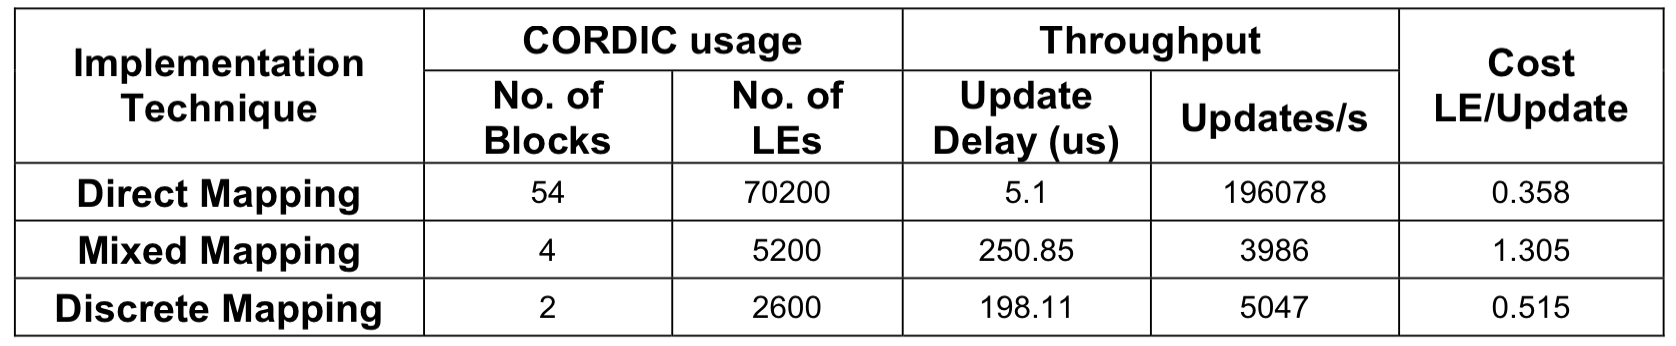
\includegraphics[width=12cm]{./figures/C03-altera_table}
     \caption{Tabla de métricas del hardware de Altera}
     \label{fig:altera_table}
\end{figure}

Entre las diferentes métricas, se encuentran las siguientes:

\begin{itemize}
\item[] \textit{Update Delay}: Tiempo requerido antes de que todas las celdas en el arreglo sistólico sean actualizadas.
\item[] \textit{Throughpu}t: Número de matrices de entrada (cada una de $M \times N$) que son procesadas por segundo ($= 1/\text{\textit{update delay}}$).
\item[] \textit{Cost}: Número de celdas básicas LE\footnote{\label{LE}Logic Element: Los elementos lógicos son las unidades más pequeñas de lógica en la arquitectura de la familia de dispositivos FPGA Cyclone III de Altera.} que ocupan las celdas CORDIC.
\end{itemize}

\subsection{Publicación de Xilinx}

\begin{itemize}
\item[] \textbf{Título}: \textit{FPGA Implementation of Matrix Inversion Using QRD-RLS Algorithm} 
\item[] \textbf{Autor/es}: Marjan Karkooti, Joseph R. Cavallaro, Chris Dick. Center for Multimedia Communication, Department of Electrical and Computer Engineering, Rice University / Xilinx
\end{itemize}

Este trabajo \cite{XilinxQR} detalla la realización de un filtro de \textit{beamforming} y fue desarrollado por un laboratorio de investigación de Xilinx en conjunto con la Universidad Rice. Su hardware utiliza dos CORDICs en \textit{vectoring mode} para cada una de las \textit{boundary cells} y la arquitectura de los mismos, a diferencia del hardware de la presente tesis, es desenrollada.

Para las \textit{internal cells}, la rotación no es implementada en hardware a través de un módulo CORDIC, sino que utiliza \textit{multiply accumulate (MAC) functional units}. Se utiliza el dispositivo FPGA Virtex 4, el cual consta de un gran arreglo de unidades MAC referidas como \textit{DSP48 slices}. Según menciona el documento, utilizar los bloques embebidos DSP48 en reemplazo de un enfoque basado en CORDIC para las \textit{internal cells} reduce la latencia de esta fase de cómputo y minimiza la cantidad de tablas de lógica FPGA (\textit{look-up tables LUTs} y registros) requeridas para la implementación. De todas maneras, se considera importante destacar el contexto de dicho tamaño dado que la arquitectura CORDIC es desenrollada.

\begin{figure}[h!]
     \centering
     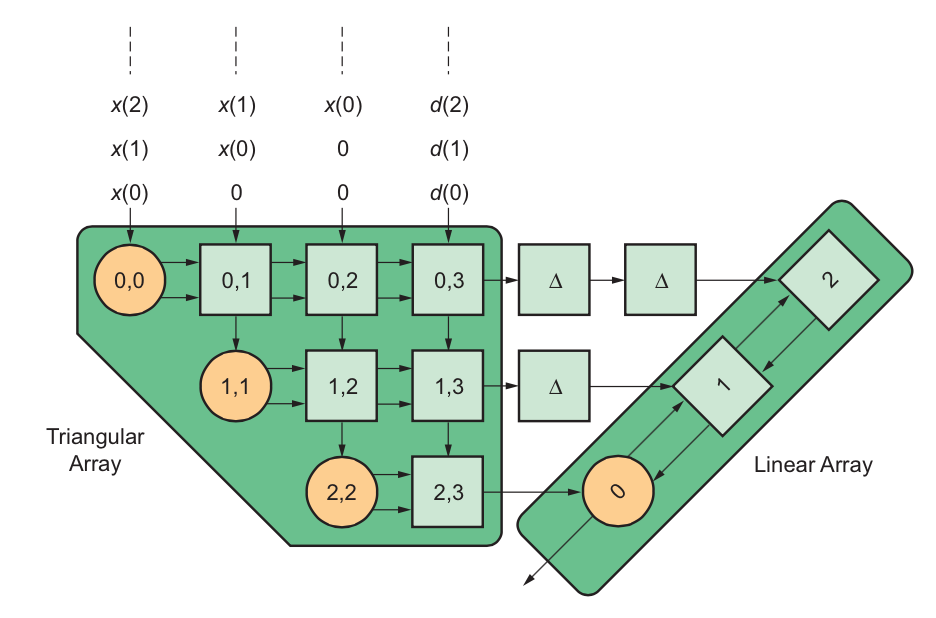
\includegraphics[width=12cm]{./figures/C03-xilinx_hardware}
     \caption{Arquitectura implementada por Xilinx}
     \label{fig:xilinx_hardware}
\end{figure}

Un dato interesante que presenta el trabajo para la comparativa es el tiempo requerido para el cálculo de la descomposición de una matriz utilizando varios valores de $M$ y $N$, entre los cuales se encuentra la matriz de $7 \times 7$. Sin embargo, no especifica la cantidad de bits de ancho de palabra utilizados.

Adicionalmente, detalla que se desarrolló un banco de pruebas con MATLAB. El script simula un objetivo dinámico y genera las muestras del patrón de radiación en campo lejano para el objetivo en movimiento. Las muestras del campo eléctrico en cada sensor se generan en MATLAB y son enviadas al procesador FPGA QRD. Se produce una nueva estimación del vector de peso conformador de haz y se envía a MATLAB para su posterior procesamiento.

\begin{figure}[h!]
     \centering
     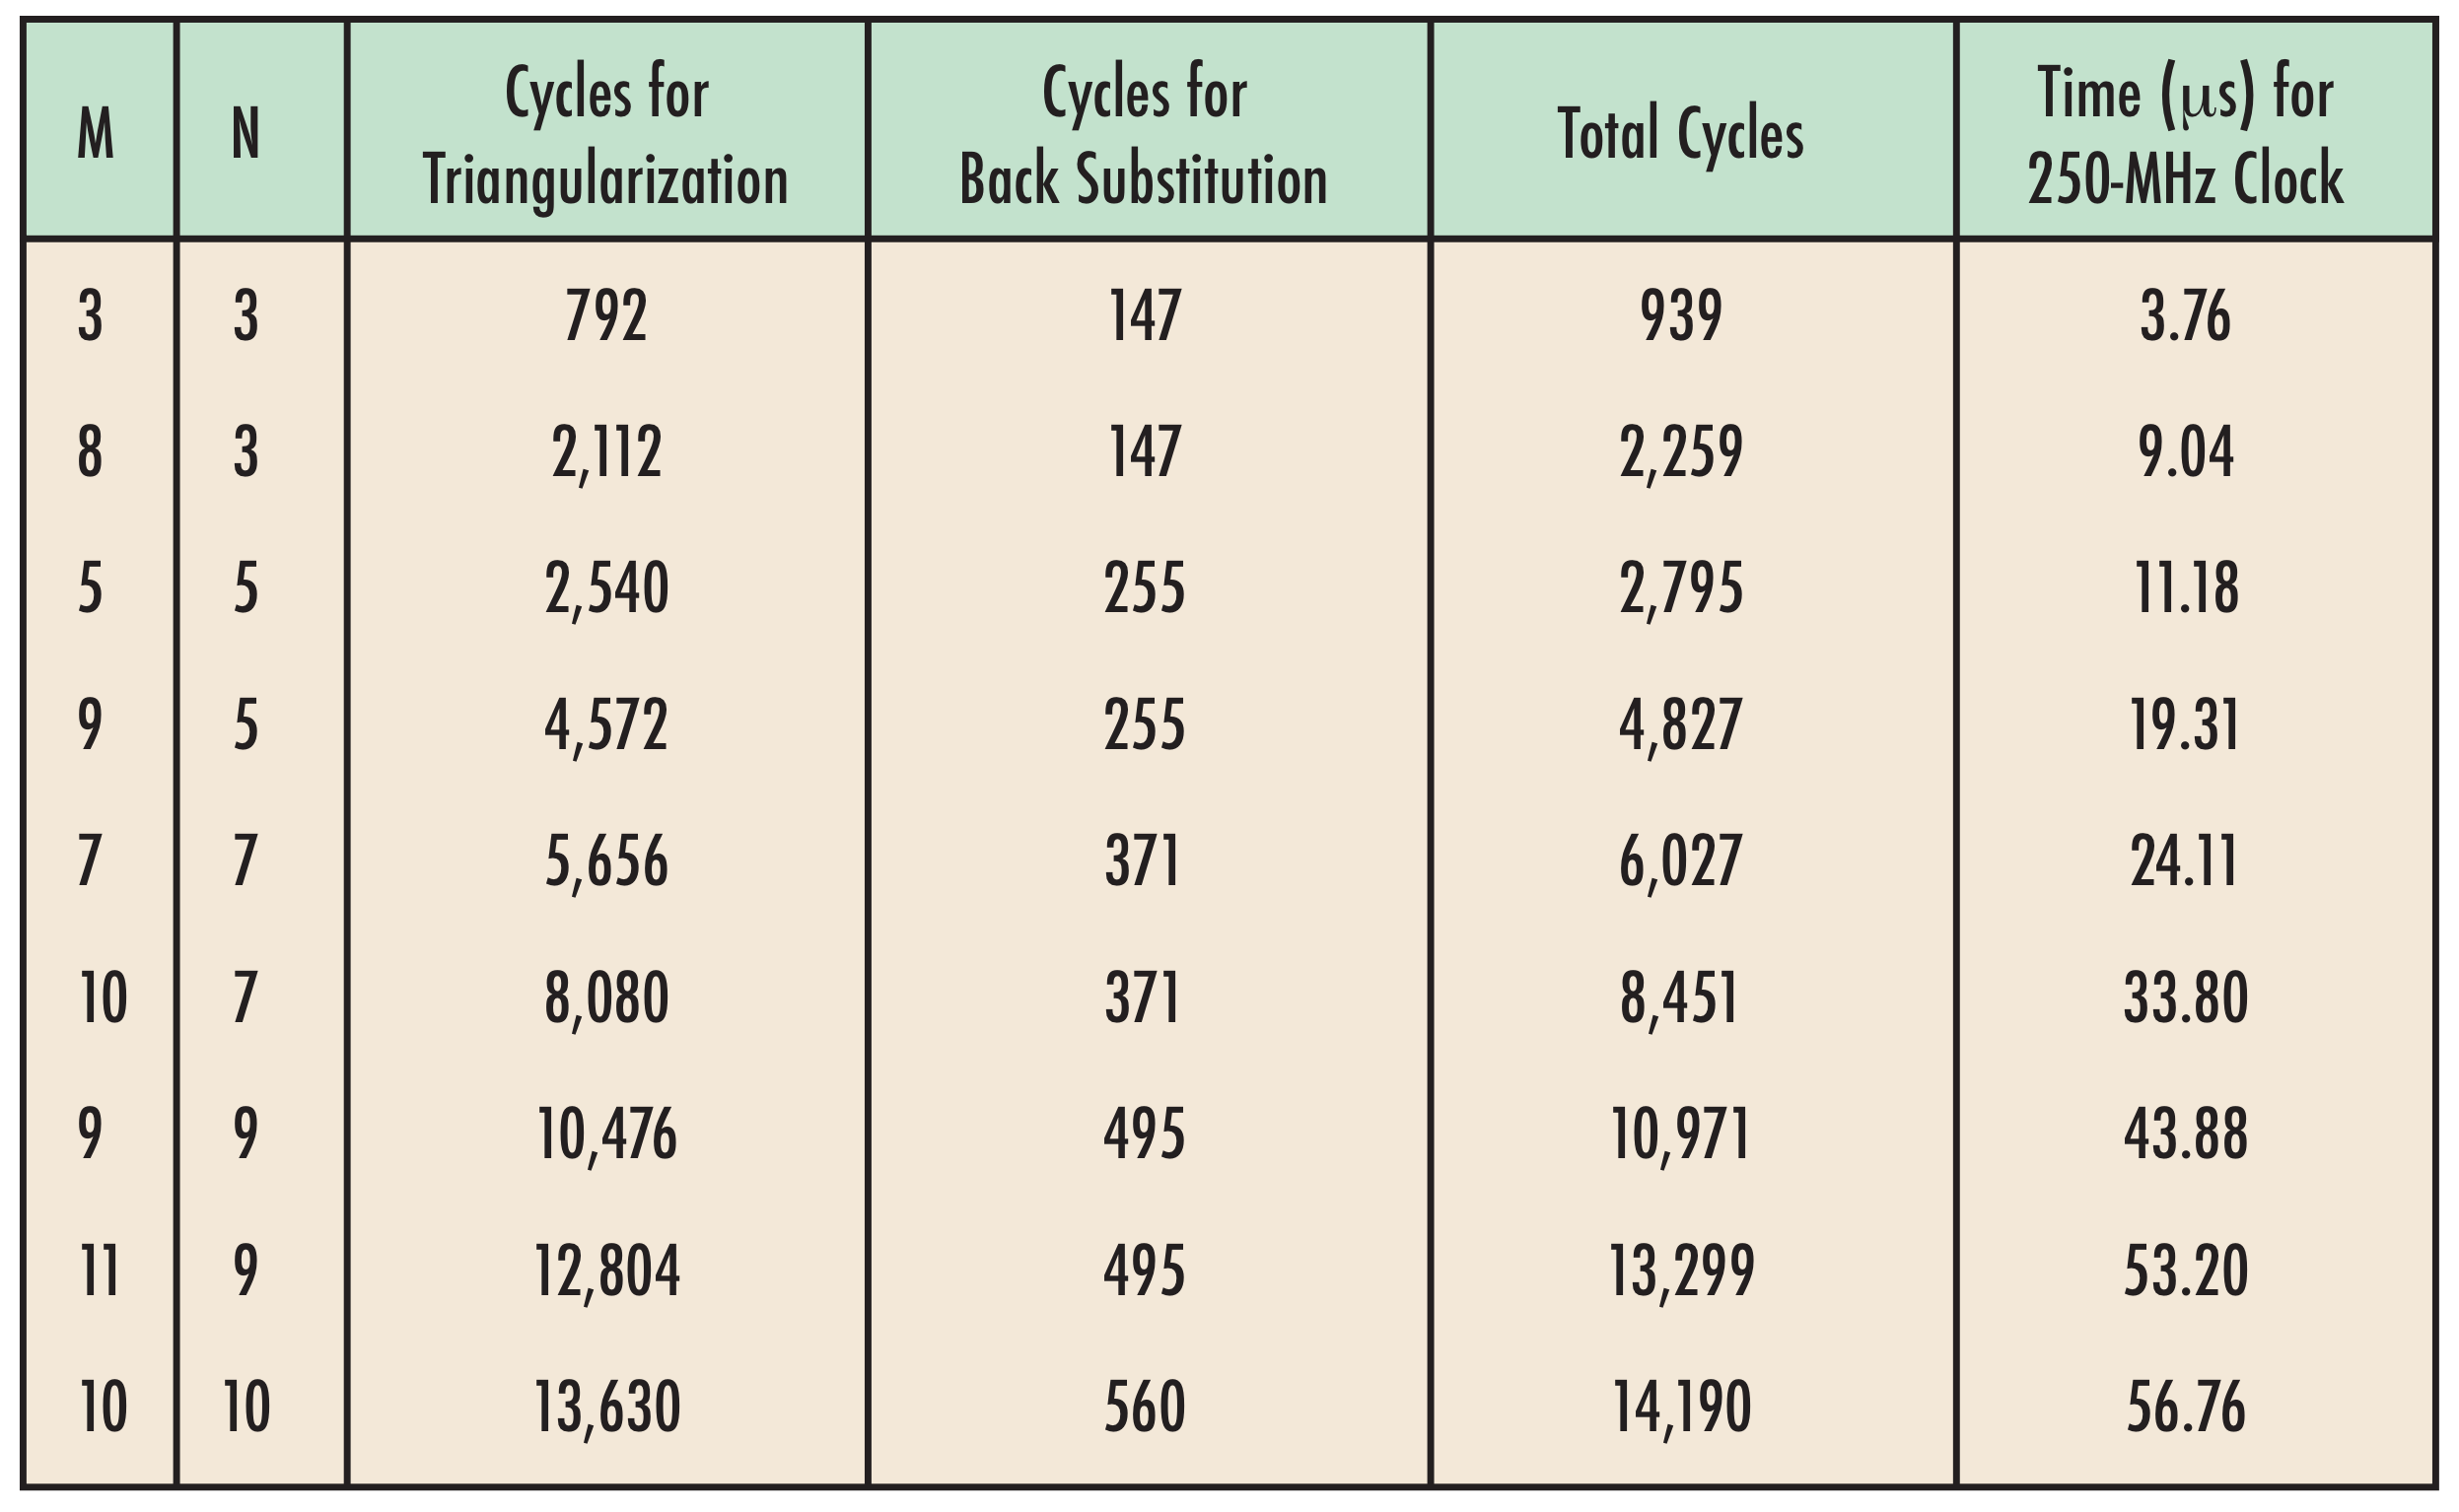
\includegraphics[width=12cm]{./figures/C03-xilinx_table}
     \caption{Tabla de métricas del hardware presentado por Xilinx}
     \label{fig:xilinx_table}
\end{figure}

\subsection{Publicación de Universidad de Victoria}

\begin{itemize}
\item[] \textbf{Título}: \textit{Fixed-Point CORDIC-Based QR Decomposition by Givens Rotations on FPGA}
\item[] \textbf{Autores}: Dongdong Chen, Mihai SIMA. Department of Electrical and Computer Engineering, University of Victoria
\end{itemize}

Este trabajo \cite{DongdongQR} contiene definiciones precisas sobre cómo fue desarrollado el hardware, cómo fue evaluado, y las diferentes métricas obtenidas. El hardware consta de un procesador de descomposición QR para matrices de $4 \times 4$, con ancho de palabra variable. Se utilizó un \textbf{mapeo directo} para desarrollar la arquitectura QR, la cual consta de un total de $21$ procesadores CORDIC.

\begin{figure}[h!]
     \centering
     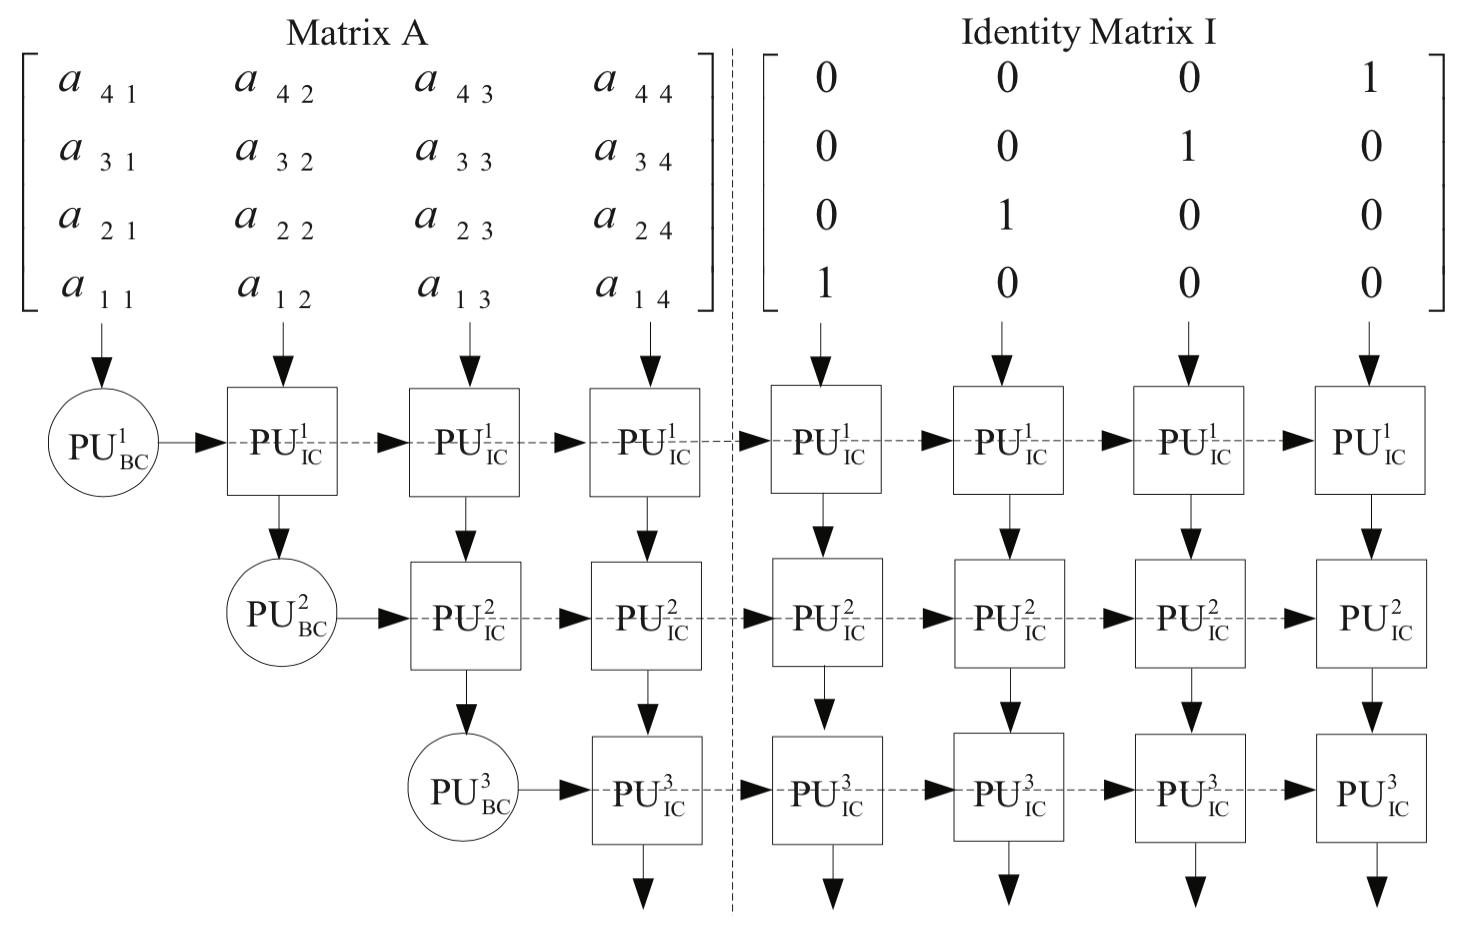
\includegraphics[width=8cm]{./figures/C03-dongdong_hardware}
     \caption{Arreglo de descomposición QR para una matriz de $4 \times 4$}
     \label{fig:dongdong_hardware}
\end{figure}

Una diferencia sustancial con la arquitectura que fue descripta, es que en ésta se agrega una sección de celdas/procesadores a derecha, la cual al ser inicializada con la matriz identidad, permite que al finalizar el cálculo se llegue al resultado de la matriz $Q^T$ (localizada en dichas celdas). Esta sección está compuesta por $3 \times 4 = 12$ celdas, siendo las $9$ celdas restantes utilizadas para el cálculo de la matriz $R$.

Se presenta un análisis teórico del \textit{timming} de la unidad, y una evaluación del error para diferentes anchos de palabra.

En forma similar al proyecto de Xilinx, desarrollaron un banco de pruebas basado en una simulación de MATLAB para contrastar resultados, utilizando un dispositivo FPGA Virtex 5 para realizar la síntesis, y sometiéndolo al cálculo de 100.000 matrices con elementos aleatorios.

Entre las métricas presentadas se encuentran distintos parámetros de evaluación del error, número de \textit{slices} ocupados, \textit{delay} de camino crítico, tiempo de procesamiento y \textit{throughput}.

\begin{figure}[h!]
     \centering
     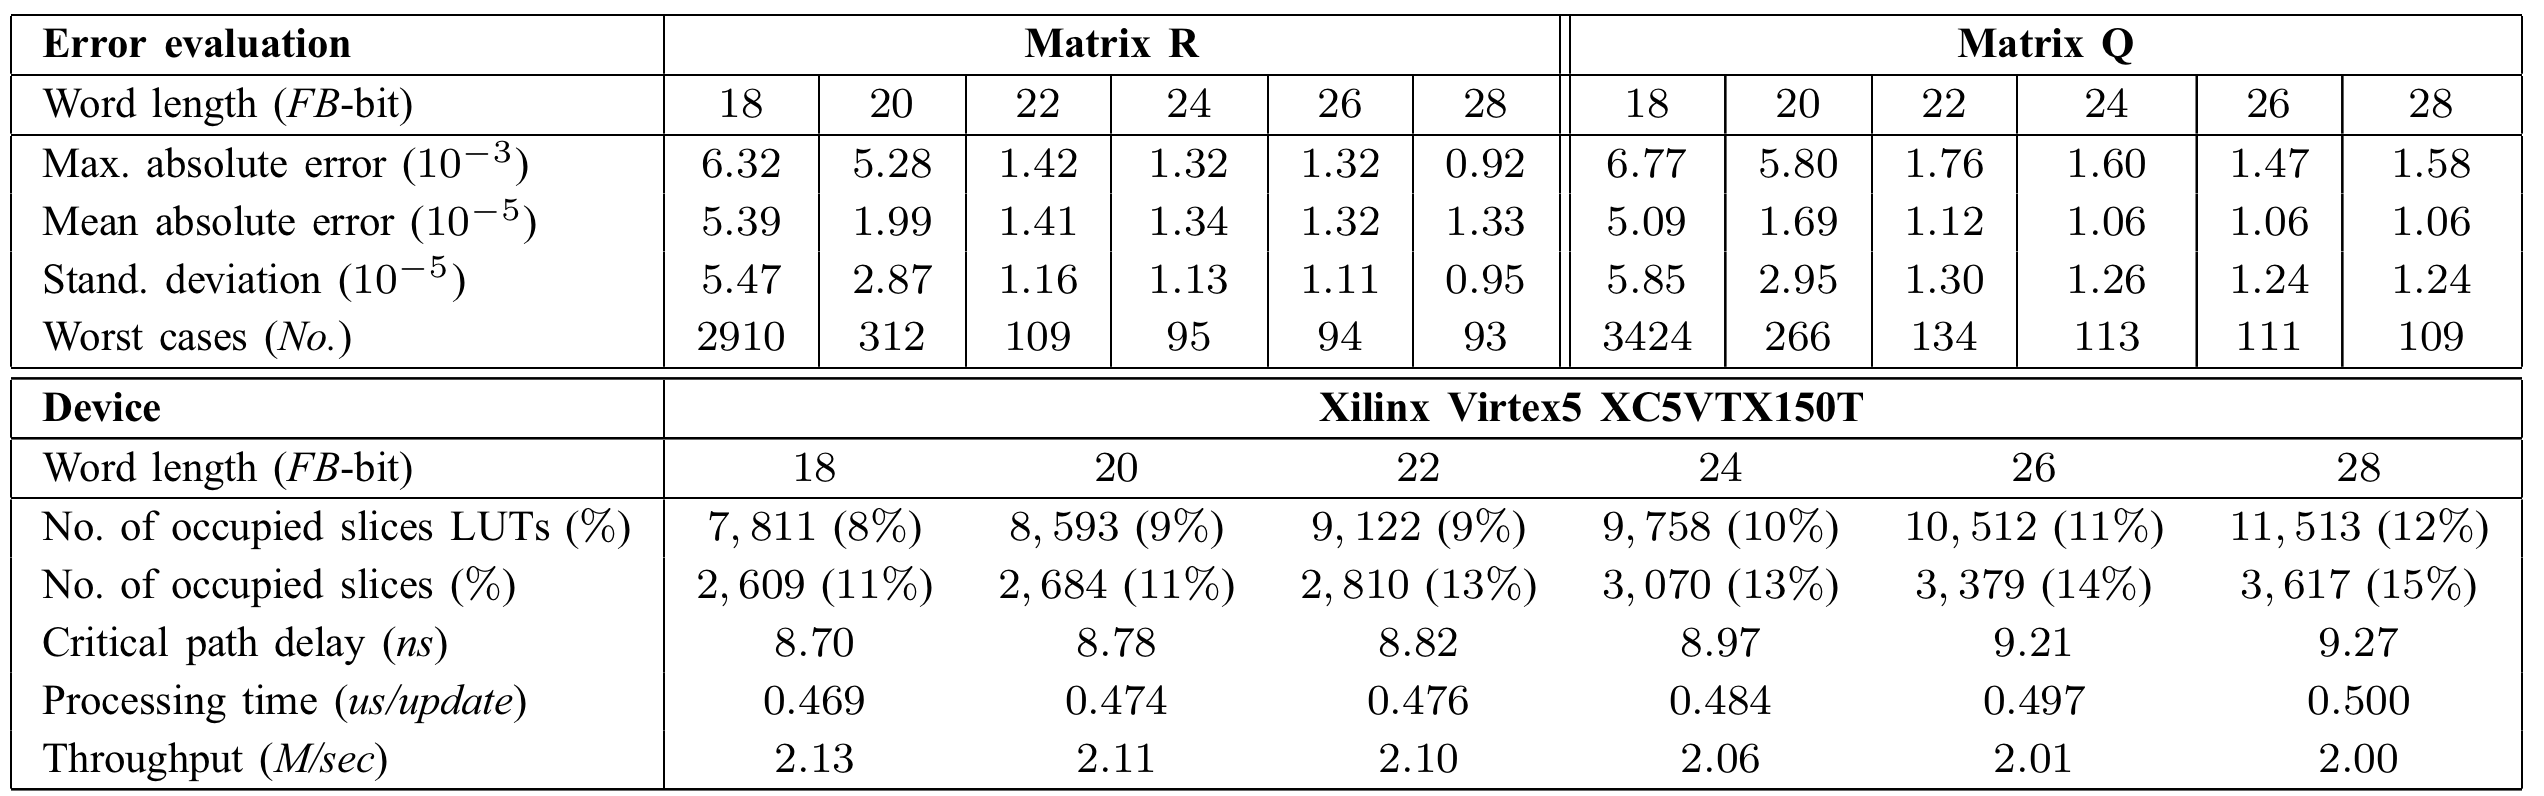
\includegraphics[width=14cm]{./figures/C03-dongdong_table}
     \caption{Tabla de métricas del hardware presentado}
     \label{fig:dongdong_table}
\end{figure}

\section{Arquitectura implementada}

La elección de la implementación utiliza RLS-QRD (algoritmo RLS a través de descomposición QR) como el sistema central para calcular adaptativamente los pesos del filtro.

A continuación se definen las premisas de la arquitectura elegida para la implementación del procesador de descomposición QR, sobre la cual se hará hincapié en el próximo capítulo:

\begin{itemize}
\item[•] \textbf{Tipo de Algoritmo:} Algoritmo Recursive Least Squares a través de descomposición QR.
\item[•] \textbf{Tipo de Rotaciones:} Rotaciones de Givens.
\item[•] \textbf{Hardware de Rotación:} CORDIC iterativo.
\item[•] \textbf{Cantidad de Procesadores de Celdas:} 4 módulos CORDIC.
\item[•] \textbf{Distribución de Celdas:} Mapeo de Walke \cite{Walke}.
\item[•] \textbf{Dimensión de la matriz:} $7 \times 7$.
\item[•] \textbf{Ancho de Palabra:} Hasta 64 \textit{bits}.
\end{itemize}